% ======================================================================
% Meta-Informationen
% ----------------------------------------------------------------------
% Zentrale Dokumentinformationen (z. B. Titel, Autor:in, Matrikelnummer)
% werden in der Datei _Meta.tex definiert und anschließend global
% im gesamten Dokument verfügbar gemacht.
% ======================================================================
% Informationen ------------------------------------------------------------
% 	Definition von globalen Parametern, die im gesamten Dokument verwendet
% 	werden können (z.B auf dem Deckblatt etc.).
% --------------------------------------------------------------------------
\newcommand{\titel}{Autonomes Landen von Drohnen in
Agrarlandschaften basierend auf
Deep-Reinforcement-Learning}
\newcommand{\art}{Bachelorarbeit}
\newcommand{\ort}{Leipzig}
\newcommand{\hochschule}{Universität Leipzig}
\newcommand{\fachgebiet}{Professur Informationsmanagement}
\newcommand{\fakultaet}{Wirtschaftswissenschaftliche Fakultät}
\newcommand{\institut}{Institut für Wirtschaftsinformatik}
\newcommand{\erstbetreuer}{Prof. Dr. Bogdan Franczyk}
\newcommand{\zweitbetreuer}{Nico Heider}

\newcommand{\autor}{Fritz Körner}
\newcommand{\matrikelnr}{3748012}
\newcommand{\email}{fk67rahe@studserv.uni-leipzig.de}
\newcommand{\telefonnummer}{+4915221457367}
\newcommand{\strasse}{Klarastraße 17}
\newcommand{\ortplz}{04229 Leipzig}

\newcommand{\eingereicht}{15. Juni 2026}

% Grad/Studiengang – anpassen, falls nötig
\providecommand{\grad}{Bachelor of Science}
\providecommand{\studiengang}{Informatik}


% Eigene Befehle
\newcommand{\todo}[1]{\textbf{\textsc{\textcolor{red}{(TODO: #1)}}}}

% Autorennamen in small caps
\newcommand{\AutorZ}[1]{\textsc{#1}}
\newcommand{\Autor}[1]{\AutorZ{\citeauthor{#1}}}

% Befehle zur semantischen Auszeichnung von Text
\newcommand{\Prozess}[1]{\textit{#1}}
\newcommand{\Webservice}[1]{\textit{#1}}
\newcommand{\Eingabe}[1]{\texttt{#1}}
\newcommand{\Code}[1]{\texttt{#1}}
\newcommand{\Datei}[1]{\texttt{#1}}
\newcommand{\Datentyp}[1]{\textsf{#1}}
\newcommand{\XMLElement}[1]{\textsf{#1}}

% Abkürzungen
\newcommand{\vgl}{Vgl.\ }
\newcommand{\ua}{\mbox{u.\,a.\ }}
\newcommand{\zB}{\mbox{z.\,B.\ }}
\newcommand{\bs}{$\backslash$}

% Einfache Anführungszeichen in texttt
\newcommand{\sq}{\textquotesingle}





% ======================================================================
% Dokumentklasse und grundlegende Layout-Einstellungen
% ----------------------------------------------------------------------
% Diese Vorlage basiert auf der KOMA-Script-Klasse "scrreprt".
% Die Option "draft" sollte ausschließlich während der Bearbeitung
% verwendet und für die finale Abgabe deaktiviert werden.
% ======================================================================
\documentclass[
	12pt,                  % Grundschriftgröße
	DIV=10,                % Satzspiegel (KOMA-Script-Berechnung)
	ngerman,               % Deutsche Sprache (Umlaute, Silbentrennung)
	a4paper,               % Papierformat
	oneside,               % Einseitiges Dokument
	titlepage,             % Separate Titelseite
	parskip=half,          % Halber Zeilenabstand zwischen Absätzen
	headings=normal,       % Reduzierte Überschriftengröße
	numbers=withendperiod, % Punkt nach Kapitel-/Abschnittsnummern
	listof=totoc,          % Verzeichnisse im Inhaltsverzeichnis
	bibliography=totoc,    % Literaturverzeichnis im Inhaltsverzeichnis
	index=totoc,           % Index im Inhaltsverzeichnis
	captions=tableheading, % Tabellenbeschriftung oberhalb
	final                  % Dokumentstatus (final/draft)
]{scrreprt}


% ======================================================================
% Benötigte Packages
% ----------------------------------------------------------------------
% Alle zusätzlichen Pakete werden in die Datei Packages.tex ausgelagert,
% um die Hauptdatei übersichtlich und wartbar zu halten.
% ======================================================================
% ======================================================================
% Encoding, Sprache, Schriften
% ======================================================================
\usepackage[utf8]{inputenc} % Bei aktuellem LaTeX oft entbehrlich, aber kompatibel.
\usepackage[T1]{fontenc}    % T1-Font-Encoding für korrekte Trennung/Umlaute.
\usepackage[ngerman,shorthands=off]{babel} % Deutsch + Deaktivierung von babel-shorthands.
\usepackage{csquotes}       % Kontextabhängige Anführungszeichen (empfohlen mit biblatex).

% Serifenschrift (Times-ähnlich) für Fließtext und Mathematik
\usepackage{newtxtext,newtxmath}

% Sans-Serif für Überschriften/Titel (Arial-Ersatz: Arimo)
\usepackage[sfdefault,scaled=0.95]{arimo}
\renewcommand{\familydefault}{\rmdefault} % Fließtext bleibt serif (Times-ähnlich).

% Einheitliche Abstände für Display-Matheumgebungen
\AtBeginDocument{%
  % Formeln als eigener Absatz (typisch mit Leerzeile davor/danach)
  \setlength{\abovedisplayskip}{10pt plus 4pt minus 5pt}%
  \setlength{\belowdisplayskip}{10pt plus 4pt minus 5pt}%
  % Formeln „kurz“ nach Einleitung im Fließtext (z. B. „… wie folgt:“)
  \setlength{\abovedisplayshortskip}{6pt plus 3pt minus 3pt}%
  \setlength{\belowdisplayshortskip}{6pt plus 3pt minus 3pt}%
  % Zeilenabstand innerhalb von align-Umgebungen
  \setlength{\jot}{2pt}%
}

% ======================================================================
% Überschriften (titlesec): Kapitel-/Abschnittsdesign
% ======================================================================
\usepackage{titlesec}

% Kapitel: 14 pt, Sans-Serif fett
\titleformat{\chapter}[hang]
  {\sffamily\bfseries\fontsize{14pt}{16pt}\selectfont}
  {\thechapter}{1em}{}
\titleformat{name=\chapter,numberless}[hang]
  {\sffamily\bfseries\fontsize{14pt}{16pt}\selectfont}{}{0pt}{}
\titlespacing*{name=\chapter,numberless}{0pt}{2pt}{10pt}

% Section/Subsection: 12 pt, Sans-Serif fett
\titleformat{\section}[hang]
  {\sffamily\bfseries\fontsize{12pt}{14pt}\selectfont}
  {\thesection}{1em}{}
\titleformat{\subsection}[hang]
  {\sffamily\bfseries\fontsize{12pt}{14pt}\selectfont}
  {\thesubsection}{1em}{}

% Subsubsection: 12 pt, Sans-Serif normal
\titleformat{\subsubsection}[hang]
  {\sffamily\fontsize{12pt}{14pt}\selectfont}
  {\thesubsubsection}{1em}{}

% ======================================================================
% Kopf- und Fußzeilen (KOMA-Script)
% ======================================================================
\usepackage[
  automark,          % Automatische Marken (Kapitel/Abschnitt) setzen
  headsepline,       % Linie unter der Kopfzeile
  plainheadsepline,  % Linie auch auf plain-Seiten
  ilines,            % Innenliegende Linienführung
  headwidth=text     % Kopfzeile auf Textbreite
]{scrlayer-scrpage}

% ======================================================================
% Grafiken
% ======================================================================
\usepackage{graphicx}
\usepackage{adjustbox}
\usepackage{wrapfig}
\graphicspath{{Bilder/}} % Standardsuchpfad für Grafiken

% ======================================================================
% Mathematik & Symbole
% ======================================================================
\usepackage{amsmath,amsfonts}
\let\openbox\relax % resolve clash: newtxmath already defines \openbox
\usepackage{amsthm}
\usepackage{dsfont}
\usepackage{nicefrac}

% ======================================================================
% Index & Nomenklatur (Abkürzungsverzeichnis)
% ======================================================================
\usepackage{makeidx}
\usepackage[intoc]{nomencl} % Nomenklatur ins Inhaltsverzeichnis aufnehmen
\let\abbrev\nomenclature
\renewcommand{\nomname}{Abkürzungsverzeichnis}
\setlength{\nomlabelwidth}{.25\hsize}
\renewcommand{\nomlabel}[1]{#1 \dotfill}
\setlength{\nomitemsep}{-\parsep}

% ======================================================================
% Tabellen: Zeilenabstände
% ======================================================================
\usepackage{setspace}
\AtBeginEnvironment{tabular}{\singlespacing} % Tabellen stets einzeilig setzen
\renewcommand{\arraystretch}{1.0}            % Zeilenhöhe innerhalb von Tabellen

% ======================================================================
% Sonstige Pakete
% ======================================================================
\usepackage{rotating}
\usepackage{float} % [H] nur sparsam verwenden (Layout kann „festkleben“).

% ======================================================================
% Quellcode (listings)
% ======================================================================
\usepackage{listings}
\usepackage{xcolor}

% Farbdefinitionen für Listings-Stil
\definecolor{codegreen}{rgb}{0,0.6,0}
\definecolor{codegray}{rgb}{0.5,0.5,0.5}
\definecolor{codepurple}{rgb}{0.58,0,0.82}
\definecolor{backcolour}{rgb}{0.95,0.95,0.92}

% Standardstil für Quellcode-Blöcke
\lstdefinestyle{mystyle}{
  backgroundcolor=\color{backcolour},
  commentstyle=\color{codegreen}\itshape,
  keywordstyle=\bfseries,
  numberstyle=\tiny\color{codegray},
  stringstyle=\ttfamily,
  basicstyle=\ttfamily\footnotesize,
  breakatwhitespace=false,
  breaklines=true,
  captionpos=b,
  keepspaces=true,
  numbers=left,
  numbersep=5pt,
  showspaces=false,
  showstringspaces=false,
  showtabs=false,
  tabsize=2
}
\lstset{style=mystyle}

% Monospace-Schrift (Courier) für Listings
\usepackage{courier}

% Wörtliche Zitate: kursiv (für längere Zitatblöcke)
\newenvironment{quoteitalic}{\begin{quote}\itshape}{\end{quote}}

% ======================================================================
% Verzeichnisse (tocloft): Abbildungen, Tabellen, Formeln, Anhang
% ======================================================================
\usepackage{tocloft}

% Einzüge in Abbildungs- und Tabellenverzeichnis entfernen
\setlength{\cftfigindent}{0pt}
\setlength{\cfttabindent}{0pt}

% Titelabstände der Verzeichnisse (wie bei nummerlosen Kapiteln: 2pt/10pt)
\setlength{\cftbeforetoctitleskip}{2pt}
\setlength{\cftaftertoctitleskip}{10pt}
\setlength{\cftbeforeloftitleskip}{2pt}
\setlength{\cftafterloftitleskip}{10pt}
\setlength{\cftbeforelottitleskip}{2pt}
\setlength{\cftafterlottitleskip}{10pt}

% Eigenes Formelverzeichnis
\newlistof{formeln}{loe}{Formelverzeichnis}
\setlength{\cftbeforeloetitleskip}{2pt}
\setlength{\cftafterloetitleskip}{10pt}
\renewcommand{\cftformelnpresnum}{}
\renewcommand{\cftformelnaftersnum}{\enspace}
\setlength{\cftformelnnumwidth}{2.25em}

% Hilfsmakro: Formel in das Formelverzeichnis eintragen
\newcommand{\eqcaption}[1]{%
  \addcontentsline{loe}{formeln}{\protect\numberline{\theequation}#1}%
}

% Überschriftenschrift der Verzeichnisse (analog Kapitelstil)
\renewcommand{\cfttoctitlefont}{\sffamily\bfseries\fontsize{14pt}{16pt}\selectfont}
\renewcommand{\cftloftitlefont}{\sffamily\bfseries\fontsize{14pt}{16pt}\selectfont}
\renewcommand{\cftlottitlefont}{\sffamily\bfseries\fontsize{14pt}{16pt}\selectfont}
\renewcommand{\cftloetitlefont}{\sffamily\bfseries\fontsize{14pt}{16pt}\selectfont}

% Anhangsverzeichnis
\newlistof{anhang}{loah}{Anhangsverzeichnis}
\setlength{\cftbeforeloahtitleskip}{2pt}
\setlength{\cftafterloahtitleskip}{10pt}
\renewcommand{\cftanhangpresnum}{Anhang~}
\renewcommand{\cftanhangaftersnum}{\enspace}
\setlength{\cftanhangnumwidth}{7em}
\renewcommand{\cftloahtitlefont}{\sffamily\bfseries\fontsize{14pt}{16pt}\selectfont}

% ======================================================================
% Hyperref & PDF-Metadaten
% ======================================================================
\usepackage[
  bookmarks,
  bookmarksopen=true,
  pdftitle={\titel},
  pdfauthor={\autor},
  pdfcreator={\autor},
  pdfsubject={\titel},
  pdfkeywords={\titel},
  colorlinks=true,
  linkcolor=black, anchorcolor=black, citecolor=black,
  filecolor=black, menucolor=black, urlcolor=black,
  plainpages=false, pdfpagelabels, hypertexnames=false, linktocpage
]{hyperref}
\usepackage{url}

% ======================================================================
% Bibliographie (biblatex, APA)
% ======================================================================
\usepackage[
  backend=biber,
  style=apa,
  sorting=nyt,
  natbib=false,
  maxcitenames=2,
  maxbibnames=20
]{biblatex}
\DeclareLanguageMapping{ngerman}{ngerman-apa}
\addbibresource{quellen.bib}

% APA-Layout: Hängender Einzug und Abstand zwischen Einträgen
\setlength{\bibhang}{1.27cm}
\setlength{\bibitemsep}{\baselineskip}

% ======================================================================
% Captions & Float-Abstände
% ======================================================================
\usepackage[font={bf,small},labelfont=bf,justification=centering]{caption}

% Abstände zwischen Objekt und Beschriftung (moderat kompakt)
\captionsetup{skip=6pt, belowskip=0pt}
\captionsetup[table]{skip=4pt}

% Abstände rund um Floats (kompakt, aber layoutstabil)
\setlength{\textfloatsep}{10pt plus 2pt minus 4pt} % Float oben/unten auf Seite
\setlength{\intextsep}{8pt plus 2pt minus 3pt}     % Float im Textfluss ([h]/[H])
\setlength{\floatsep}{8pt plus 2pt minus 3pt}      % Zwischen zwei Floats

\DeclareCaptionLabelFormat{anhangnonum}{#1}

% ======================================================================
% Tabellen & Layout-Helfer
% ======================================================================
\usepackage{longtable}
\usepackage{array}
\usepackage{ragged2e}
\usepackage{lscape}
\usepackage{booktabs}
\usepackage{supertabular}
\usepackage[table,xcdraw]{xcolor}
\newcolumntype{w}[1]{>{\raggedleft\arraybackslash}p{#1}}

% Listen und Fußnoten in Tabellen
\usepackage{paralist}
\usepackage{tablefootnote}

% ======================================================================
% Algorithmen
% ======================================================================
\usepackage[linesnumbered,ruled]{algorithm2e}
\SetKwInput{KwInput}{Input}
\SetKwInput{KwOutput}{Output}

% ======================================================================
% Hinweis zur Layoutstabilität
% ----------------------------------------------------------------------
% Keine Neu-Definition von figure/table/equation-Umgebungen, da dies
% Abstände und Nummerierungen unerwartet beeinflussen kann.
% ======================================================================



% Keine erzwungene vertikale Ausdehnung der Seiten
\raggedbottom


% Kein Absatzeinzug (auch nicht nach mathematischen Umgebungen)
\AtBeginDocument{%
  \setlength{\parindent}{0pt}
}


% ======================================================================
% Definition für Anhangsabschnitte
% ----------------------------------------------------------------------
% Erstellt einen neuen Anhangsabschnitt (A, B, C, ...), setzt die
% Medienzähler zurück und sorgt für korrekte Einträge im Anhangsverzeichnis.
% ======================================================================
\makeatletter
\newcommand{\appsection}[1]{%
  \clearpage
  \refstepcounter{section}%
  \setcounter{figure}{0}%
  \chapter*{\thesection\quad #1}%
  \addcontentsline{loah}{anhang}{\protect\numberline{\thesection}#1}%
}
\makeatother


% ======================================================================
% Index- und Abkürzungsverzeichnis aktivieren
% ----------------------------------------------------------------------
% Beispiel für die Index-Erstellung:
% makeindex Masterarbeit.nlo -s nomencl.ist -o Masterarbeit.nls
% ======================================================================
\makeindex
\makenomenclature


% ======================================================================
% Kopf- und Fußzeilen, Seitenränder etc.
% ----------------------------------------------------------------------
% Definition des Seitenstils in einer separaten Datei.
% ======================================================================
% ======================================================================
% Zeilenabstand und Absatzlayout
% ======================================================================
\setstretch{1.5} % 1,5-zeiliger Zeilenabstand im Fließtext
\AtBeginDocument{%
  \setlength{\parindent}{0pt}% kein Absatzeinzug
  \setlength{\parskip}{4pt plus 1pt minus 1pt}% Abstand zwischen Absätzen (leicht flexibel)
}


% ======================================================================
% Seitenränder (geometry)
% ======================================================================
\usepackage{geometry}
\geometry{paper=a4paper,left=30mm,right=25mm,top=25mm,bottom=15mm}

% Alternative Rand-Einstellungen (nur bei Bedarf verwenden)
% \geometry{paper=a4paper,left=35mm,right=25mm,top=25mm,bottom=25mm}


% ======================================================================
% Kopf- und Fußzeilen (scrlayer-scrpage)
% ----------------------------------------------------------------------
% Zentraler Seitenstil: Kopfzeile mit Headmark und Seitenzahl,
% Fußzeile vollständig leer.
% ======================================================================
\clearpairofpagestyles

% Kopfzeile: innen/links Headmark (kursiv), außen/rechts Seitenzahl
\ihead[\textit{\headmark}]{\textit{\headmark}}
\ohead[\pagemark]{\pagemark}

% Fußzeile deaktivieren
\lefoot{}\cefoot{}\refoot{}
\lofoot{}\cofoot{}\rofoot{}

% Schrift im Kopf: normal (nicht smallcaps o. ä.)
\renewcommand{\headfont}{\normalfont}

% Abmessungen/Abstände der Kopf- und Fußbereiche
\setlength{\headheight}{8mm}
\setlength{\headsep}{4mm}
\setlength{\footskip}{8mm}

% Kapitelanfangsseiten (plain) an den Standard-Seitenstil anpassen
% Hinweis: Nach dem Laden von scrlayer-scrpage ausführen.
\makeatletter
\let\ps@plain\ps@scrheadings
\makeatother

% Kopfbreite exakt auf Textbreite setzen
\AtBeginDocument{\KOMAoptions{headwidth=text}}


% ======================================================================
% Kapitelstart: vertikaler Abstand (KOMA-Script)
% ----------------------------------------------------------------------
% Schiebt die Kapitelüberschrift näher an den oberen Rand.
% Vorsicht: Zu große negative Werte können Layout-Probleme verursachen.
% ======================================================================
\renewcommand*\chapterheadstartvskip{\vspace*{-1.0cm}}


% ======================================================================
% Typografie: Satzzeichenabstände
% ----------------------------------------------------------------------
% Aktiviert „französischen Abstand“: einheitliche Abstände nach Satzzeichen.
% ======================================================================
\frenchspacing


% ======================================================================
% Schusterjungen und Hurenkinder vermeiden (Witwen/Waisen)
% ======================================================================
\clubpenalty=10000
\widowpenalty=10000
\displaywidowpenalty=10000


% ======================================================================
% Quellcode-Ausgabe (listings): Grundlayout
% ======================================================================

% Beispiel-Optionen (bei Bedarf aktivieren/anpassen)
% \lstset{numbers=left, numberstyle=\tiny, numbersep=5pt, breaklines=true}
% \lstset{emph={square}, emphstyle=\color{red}, emph={[2]root,base}, emphstyle={[2]\color{blue}}}

% Hintergrundfarbe für Listings
\definecolor{gray}{rgb}{0.9,0.9,0.9}

% Standard-Listing-Einstellungen
\lstset{
  basicstyle=\small\ttfamily,language={[LaTeX]TeX},
  numbersep=5mm,
  numbers=left,
  numberstyle=\tiny,
  breaklines=true,
  framexleftmargin=8mm,
  xleftmargin=8mm,
  backgroundcolor=\color{gray},
  captionpos=b
}


% ======================================================================
% Fußnoten: fortlaufende Nummerierung über Kapitel hinweg
% ======================================================================
\counterwithout{footnote}{chapter}


% ======================================================================
% Theorem-Umgebungen
% ======================================================================
\newtheorem{definition}{Definition}


% ======================================================================
% Abstände um Überschriften (titlesec)
% ----------------------------------------------------------------------
% Format: \titlespacing*{<Befehl>}{<linker Einzug>}{<Abstand davor>}{<Abstand danach>}
% ======================================================================
\titlespacing*{\chapter}{0pt}{-5pt}{12pt}
\titlespacing*{\section}{0pt}{12pt}{6pt}
\titlespacing*{\subsection}{0pt}{10pt}{4pt}
\titlespacing*{\subsubsection}{0pt}{8pt}{4pt}

% Nummerlose Kapitel (z. B. Abstract) separat definieren
\titlespacing*{name=\chapter,numberless}{0pt}{2pt}{10pt}



% Eigene Silbentrennungsregeln
% ======================================================================
% Manuelle Silbentrennung
% ----------------------------------------------------------------------
% Erzwingt korrekte Worttrennungen für Begriffe, die von LaTeX
% nicht zuverlässig oder nicht wie gewünscht getrennt werden.
% Die Trennstellen werden mit Bindestrichen markiert.
% ======================================================================

\hyphenation{Trenn-bar-es}
\hyphenation{Re-gu-la-ri-sie-rung}
\hyphenation{ML-An-wen-dun-gen}



% ======================================================================
% Dokumentbeginn
% ----------------------------------------------------------------------
% Der eigentliche Inhalt beginnt hier. Kapitel und Seiten werden in
% separate Dateien ausgelagert und an dieser Stelle eingebunden.
% ======================================================================
\begin{document}


% Nummerierung bis einschließlich subsubsection aktivieren
\setcounter{secnumdepth}{3}
\setcounter{tocdepth}{3}


% ======================================================================
% Deckblatt (ohne Kopf- und Fußzeilen)
% ======================================================================
\begingroup
  \pagestyle{empty}
  % ======================================================================
% Deckblatt
% ----------------------------------------------------------------------
% Gestaltung der Titelseite ohne Kopf- und Fußzeilen.
% Enthält Logo, institutionelle Angaben, Titel der Arbeit sowie
% persönliche Angaben der Autorin / des Autors.
% ======================================================================

\thispagestyle{empty}
\begin{titlepage}

% ======================================================================
% Farbdefinition
% ----------------------------------------------------------------------
% Definiert einen mittleren Grauton für dezente Hervorhebungen
% (z. B. Betreuer:innen, persönliche Angaben).
% ======================================================================
\definecolor{mittelgrau}{gray}{0.4}


% ======================================================================
% Logo (oben links)
% ----------------------------------------------------------------------
% Einbindung des Universitätslogos mit fester Breite.
% ======================================================================
\noindent
\includegraphics[width=0.4\textwidth]{Bilder/Uni-L.png}
\vspace{0.8ex}


% ======================================================================
% Institutionelle Angaben (links unter dem Logo)
% ----------------------------------------------------------------------
% Fakultät, Institut, Fachgebiet sowie Erst- und Zweitbetreuung.
% Betreuer:innen werden kursiv und in Graustufe dargestellt.
% ======================================================================
{\raggedright
\fakultaet\\[0.6ex]
\institut\\[0.6ex]
\fachgebiet\\[0.6ex]
{\itshape \textcolor{mittelgrau}{\erstbetreuer} \\[0.6ex]
\textcolor{mittelgrau}{\zweitbetreuer}}\par
}


% ======================================================================
% Vertikaler Abstand zum Mittelblock
% ======================================================================
\vspace{28mm}


% ======================================================================
% Mittelblock
% ----------------------------------------------------------------------
% Enthält Thema, Titel der Arbeit sowie Art der Arbeit,
% angestrebten akademischen Grad und Studiengang.
% ======================================================================
\begin{center}
  Thema\\[1.2ex]
  {\large\textit{\titel}}\\[4.2ex]
  \art\ zur Erlangung des akademischen Grades\\
  \grad\ -- \textit{\studiengang}
\end{center}

\vfill


% ======================================================================
% Fußbereich: Persönliche Angaben (unten links)
% ----------------------------------------------------------------------
% Name, Matrikelnummer, Kontaktdaten und Anschrift der Autorin /
% des Autors, tabellarisch ausgerichtet.
% ======================================================================
\begin{tabular}{@{}l l}
  vorgelegt von:   & \textcolor{mittelgrau}{\textit{\autor}} \\ [2.4ex]
  Matrikelnummer: & \textcolor{mittelgrau}{\textit{\matrikelnr}} \\ [2.4ex]
  E-Mail-Adresse: & \textcolor{mittelgrau}{\textit{\email}} \\ [2.4ex]
  Telefonnummer:  & \textcolor{mittelgrau}{\textit{\telefonnummer}} \\ [2.4ex]
  Anschrift:      & \textcolor{mittelgrau}{\textit{\strasse}} \\ [0.6ex]
                  & \textcolor{mittelgrau}{\textit{\ortplz}}
\end{tabular}


% ======================================================================
% Abgabedatum
% ----------------------------------------------------------------------
% Ort und Datum der Einreichung am unteren Seitenrand.
% ======================================================================
\vspace{8mm}

\noindent \ort, den \textcolor{mittelgrau}{\eingereicht}

\end{titlepage}

\endgroup


% ======================================================================
% Abstract / Zusammenfassung
% ----------------------------------------------------------------------
% Ohne Kopfzeile, Fußzeile mit Seitenzahl bleibt erhalten.
% ======================================================================
\begingroup
  \pagestyle{empty}
  \chapter*{Zusammenfassung}
\thispagestyle{empty}
Die autonome Landung von Drohnen in hindernisreichen Umgebungen erfordert die gleichzeitige Bewältigung von Zielnavigation und Hindernisvermeidung. Bestehende Ansätze behandeln diese Teilaufgaben überwiegend getrennt, und insbesondere in natürlichen Umgebungen mit dichter Vegetation fehlen integrierte Lösungen. Die vorliegende Arbeit untersucht, inwiefern ein Reinforcement-Learning-basierter Ansatz eine autonome Drohne befähigen kann, mithilfe einer minimalen Sensorkonfiguration aus Tiefenkamera und propriozeptivem Zustandsvektor in solchen Umgebungen sicher zu landen. Dazu wird ein Agent mit einer CNN-MLP-Architektur mittels Proximal Policy Optimization in einer simulierten Korridorumgebung mit 3D-Hindernissen im Genesis-Physiksimulator trainiert. Ein kaskadierter PID-Regler überführt die gelernten Positionsbefehle in Motorsteuerungssignale. Die Evaluation erfolgt zweiphasig: In Phase~1 erreicht der Agent in der Trainingsumgebung mit ungesehenen Hindernissen eine Erfolgsrate von 98,4\,\%. In Phase~2 wird die gelernte Strategie im Zero-Shot-Transfer auf eine photogrammetrische Weinbergumgebung übertragen. Hier zeigt sich eine deutliche Leistungsreduktion (10,4\,\% Erfolgsrate bei 0,5\,m Landeradius), wobei der Agent das Ziel zuverlässig anfliegt, jedoch an der terminalen Präzisionslandung scheitert. Das Training erweist sich als instabil: Nur vier von sechs Seeds konvergieren, wobei drei davon nach Erreichen des Optimums einen abrupten Strategiekollaps zeigen, was ein gezieltes Early Stopping erfordert. Die Ergebnisse belegen, dass RL mit minimaler Sensorik die kombinierte Aufgabe in der Trainingsumgebung löst. Der Transfer auf realistische Vegetation ist eingeschränkt möglich, wobei die Leistungsgrenzen in der Trainingsdiversität und fehlender zeitlicher Integration der Beobachtungen liegen.

\emph{Schlüsselwörter:} \\
Reinforcement Learning, autonome Drohnenlandung, Hindernisvermeidung, Tiefensensorik, Proximal Policy Optimization, Genesis-Simulator
\endgroup


% Ab hier gilt wieder der reguläre Seitenstil
\pagestyle{scrheadings}


% ======================================================================
% Römische Seitennummerierung für Vorspann
% ======================================================================
\pagenumbering{Roman}


% ======================================================================
% Inhaltsverzeichnis
% ======================================================================
\cleardoublepage
\phantomsection
\addcontentsline{toc}{chapter}{Inhaltsverzeichnis}
\tableofcontents


% ======================================================================
% Abbildungs- und Tabellenverzeichnisse
% ======================================================================
\cleardoublepage
\phantomsection
\addcontentsline{toc}{chapter}{\listfigurename}
\listoffigures

\cleardoublepage
\phantomsection
\addcontentsline{toc}{chapter}{\listtablename}
\listoftables


% ======================================================================
% Formelverzeichnis
% ======================================================================
\cleardoublepage
\phantomsection
\addcontentsline{toc}{chapter}{Formelverzeichnis}
\listofformeln


% ======================================================================
% Abkürzungsverzeichnis
% ======================================================================
\abbrev{AABB}{Axis-Aligned Bounding Box}
\abbrev{CNN}{Convolutional Neural Network}
\abbrev{GNSS}{Global Navigation Satellite System}
\abbrev{GPU}{Graphics Processing Unit}
\abbrev{GSO}{Google Scanned Objects}
\abbrev{HPC}{High-Performance Computing}
\abbrev{IMU}{Inertial Measurement Unit}
\abbrev{MDP}{Markov Decision Process}
\abbrev{ML}{Machine Learning}
\abbrev{MLP}{Multilayer Perceptron}
\abbrev{PID}{Proportional-Integral-Derivative}
\abbrev{PPO}{Proximal Policy Optimization}
\abbrev{RL}{Reinforcement Learning}
\abbrev{URDF}{Unified Robot Description Format}


\begingroup
  \setlength{\parskip}{0pt}
  \printnomenclature
\endgroup
\label{sec:Glossar}
\cleardoublepage


% ======================================================================
% Arabische Seitennummerierung für den Hauptteil
% ======================================================================
\clearpage
\pagenumbering{arabic}


% ======================================================================
% Hauptinhalt
% ======================================================================
\chapter{Einleitung}
\label{cha:Einleitung}

\section{Motivation und Problemstellung}
Die Landwirtschaft steht vor wachsenden Herausforderungen: Der Klimawandel führt zu erhöhtem Schädlingsdruck, veränderten Niederschlagsmustern und sinkenden Erträgen \autocite{calvinIPCC2023Climate2023, hultgrenImpactsClimateChange2025, ClimateChangeTrends}, während eine wachsende Weltbevölkerung und zunehmender Fachkräftemangel den Produktionsdruck zusätzlich verschärfen \autocite{foodandagricultureorganizationoftheunitednationsFutureFoodAgriculture2017, WorldPopulationProspects, duckettAgriculturalRoboticsFuture2018}. Im Rahmen der digitalen Landwirtschaft bieten Drohnen (unbemannte Luftfahrzeuge) vielversprechende Lösungsansätze \autocite{bassoDigitalAgricultureDesign2020}: Sie ermöglichen unter anderem die gezielte Ausbringung von Pflanzenschutzmitteln sowie großflächiges Crop-Monitoring mittels Remote~Sensing \autocite{mashoriRemoteSensingUAVs2026, radoglou-grammatikisCompilationUAVApplications2020} und können so dazu beitragen, die Landwirtschaft effizienter und resilienter zu gestalten \autocite{undeExpandingRoleMultirotor2025, guebsi2024drones}.

Trotz umfangreicher Forschung zu Drohnensystemen bleibt autonomes Landen eine offene Herausforderung \autocite{amendolaDroneLandingReinforcement2024}. Unfallfreies Landen ist für die meisten Flugmissionen essentiell; gleichzeitig erfordern die vielfältigen Landeszenarien jeweils angepasste Lösungen. Bisherige Ansätze reichen von Global Navigation Satellite System (GNSS)-gestützter Positionierung \autocite{patrikGNSSbasedNavigationSystems2019} über markerbasierte visuelle Verfahren \autocite{wubbenAccurateLandingUnmanned2019} bis hin zu markerfreien Systemen, die Landezonen eigenständig aus Sensordaten ableiten \autocite{bartolomeiAutonomousEmergencyLanding2022}. Dabei zeigt sich eine wiederkehrende Einschränkung: Systeme zur Hindernisvermeidung navigieren erfolgreich durch komplexe Umgebungen, ohne gezielt zu landen \autocite{loquercioLearningHighspeedFlight2021, xuNavRLLearningSafe2024}, während Landesysteme überwiegend in hindernisfreien Szenarien operieren \autocite{polvaraSimtoRealQuadrotorLanding2020, ladoszAutonomousLandingMoving2024}. Die Kombination beider Teilaufgaben, Präzisionslandung mit gleichzeitiger Hindernisvermeidung, ist insbesondere in natürlichen Umgebungen mit dichter Vegetation bislang kaum untersucht. Weinberge sind ein konkretes Beispiel solcher Umgebungen: Reihenabstände von typischerweise 1,5 bis 2\,m und dichtes Blattwerk erzeugen beengte Platzverhältnisse, die eine autonome Landung zwischen den Reihen erheblich erschweren.

Reinforcement Learning (RL) hat sich in jüngerer Zeit als wirksame Lösungsstrategie für Drohnenaufgaben etabliert \autocite{kaufmannChampionlevelDroneRacing2023, hodgeDeepReinforcementLearning2021, amendolaDroneLandingReinforcement2024}: Ein RL-Agent erlernt eine Steuerungsstrategie durch Interaktion mit einer simulierten Umgebung, ohne dass ein explizites Umgebungsmodell oder manuell definierte Steuerungsregeln benötigt werden. In Kombination mit Convolutional Neural Networks (CNNs) können aufgabenrelevante Merkmale direkt aus Sensordaten extrahiert werden \autocite{mnihHumanlevelControlDeep2015}, was eine bildbasierte Hindernisvermeidung ohne manuelle Merkmalsdefinition ermöglicht.

Da Drohnen engen Gewichts- und Energiebeschränkungen unterliegen \autocite{semerikovVisionBasedAutonomousUAV2025}, beschränkt sich die vorliegende Arbeit auf eine minimale Sensorkonfiguration aus Tiefenkamera und propriozeptivem Zustandsvektor und setzt auf einen lernbasierten Ansatz, um diese begrenzte Sensorik für die autonome Landung in hindernisreichen Umgebungen auszunutzen.

\section{Zielstellung}

Ziel der Arbeit ist die Entwicklung eines Reinforcement-Learning-basierten Verfahrens, das eine autonome Multirotor-Drohne befähigt, mithilfe lokaler Tiefensensorik in einer hindernisreichen Umgebung sicher zu landen. Das System kombiniert einen propriozeptiven Zustandsvektor mit tiefenbildbasierter Umgebungswahrnehmung, um Hindernisse während des Landevorgangs zu erkennen und ihnen auszuweichen. Die Leistungsfähigkeit des trainierten Agenten wird anhand einer abstrakten Trainingsumgebung evaluiert und anschließend im Zero-Shot-Transfer, also ohne erneutes Training in der Zielumgebung, auf eine Umgebung mit realistischer Vegetationsstruktur getestet.

Dadurch ergeben sich folgende Fragestellungen:

\minisec{Hauptfragestellung}
Inwiefern kann ein Reinforcement-Learning-basierter Ansatz eine autonome Drohne befähigen, mithilfe lokaler Tiefensensorik in hindernisreichen Umgebungen sicher zu landen?

\minisec{Nebenfragestellungen}
\begin{enumerate}
	\item Wie leistungsfähig ist der trainierte Agent in der Trainingsumgebung, und welche Faktoren begrenzen die Erfolgsrate?
	\item In welchem Maß lässt sich die erlernte Navigationsleistung auf eine geometrisch verschiedenartige Umgebung mit realistischer Vegetationsstruktur übertragen?
	\item Welche Leistungslücke besteht zwischen einem lernbasierten Agenten mit lokaler Sensorik und einem Pfadplaner mit vollständiger Umgebungsinformation?
\end{enumerate}

\section{Aufbau der Arbeit}

Kapitel~\ref{cha:Fachliche Grundlagen} führt die für diese Arbeit relevanten Grundlagen ein: die theoretischen Grundlagen des Reinforcement Learning von der MDP-Formulierung über Wertfunktionen bis hin zu Proximal Policy Optimization, Convolutional Neural Networks zur Merkmalsextraktion aus Bilddaten sowie achsenparallele Bounding Boxes zur Kollisionserkennung. Kapitel~\ref{cha:Stand der Forschung} gibt einen Überblick über bestehende Ansätze zur autonomen Drohnenlandung und Hindernisvermeidung und identifiziert die Forschungslücke, die diese Arbeit adressiert. Kapitel~\ref{cha:Methodik} beschreibt das entwickelte System, einschließlich der MDP-Formulierung, der CNN-MLP-Architektur, der simulierten Trainingsumgebung und des zweiphasigen Evaluationsprotokolls. Kapitel~\ref{cha:Ergebnisse} präsentiert die experimentellen Ergebnisse beider Evaluationsphasen sowie den Vergleich mit einem klassischen Pfadplaner. Kapitel~\ref{cha:Diskussion} interpretiert die Ergebnisse im Kontext der Forschungsfragen und diskutiert Limitationen des Ansatzes. Kapitel~\ref{cha:Fazit und Ausblick} fasst die zentralen Erkenntnisse zusammen und skizziert Perspektiven für weiterführende Arbeiten.

\chapter{Fachliche Grundlagen}
\label{cha:Fachliche Grundlagen}

Dieses Kapitel führt die theoretischen Grundlagen ein, auf denen das in dieser Arbeit entwickelte System aufbaut. Abschnitt~\ref{sec:reinforcement_learning} behandelt Reinforcement Learning als Lernparadigma und formalisiert das Problem als Markov Decision Process. Abschnitt~\ref{sec:ppo} stellt Lösungsverfahren vor, ausgehend von tabellarischen Methoden über Funktionsapproximation bis hin zu Proximal Policy Optimization, dem in dieser Arbeit eingesetzten Trainingsalgorithmus. Abschnitt~\ref{sec:cnn} beschreibt Convolutional Neural Networks als Architektur zur Verarbeitung räumlicher Sensordaten. Abschnitt~\ref{sec:aabb} definiert achsenparallele Begrenzungsboxen, die in dieser Arbeit zur Kollisionserkennung verwendet werden.

\section{Reinforcement Learning}
\label{sec:reinforcement_learning}

Reinforcement Learning bezeichnet das Lernen aus Interaktionen mit einer Umgebung, um ein Ziel zu erreichen. Ein Agent wählt in aufeinanderfolgenden Situationen Aktionen und erhält dafür numerische Belohnungen. Aus diesen Erfahrungen muss er eigenständig ableiten, welche Aktionen nicht nur unmittelbar, sondern auch langfristig den höchsten Ertrag erzielen. Sofern nicht anders angegeben, folgt die Darstellung in diesem Abschnitt \textcite{suttonReinforcementLearningIntroduction2020}.

\subsection{Markov Decision Process}
\label{subsec:mdp}
Ein \Fachbegriff{Markov Decision Process} (MDP) ist ein Modell, mit dem Reinforcement Learning Probleme präzise formalisiert werden können. Der Lerner und Entscheider wird als \NeuerBegriff{Agent} bezeichnet; alles außerhalb, womit der Agent interagiert und was er nicht willkürlich verändern kann, bildet die \NeuerBegriff{Umgebung}.

Die Interaktion zwischen Agent und Umgebung erfolgt in diskreten Zeitschritten $t = 0, 1, 2, \dots$. In jedem Schritt beobachtet der Agent einen \NeuerBegriff{Zustand} $S_t \in \mathcal{S}$, wählt auf dessen Grundlage eine \NeuerBegriff{Aktion} $A_t \in \mathcal{A}$ und erhält einen Zeitschritt später eine numerische \NeuerBegriff{Belohnung} $R_{t+1} \in \mathcal{R}$ sowie einen neuen Zustand $S_{t+1}$ (Abbildung~\ref{fig:mdp_agent_environment}).

\begin{figure}[H]
    \centering
    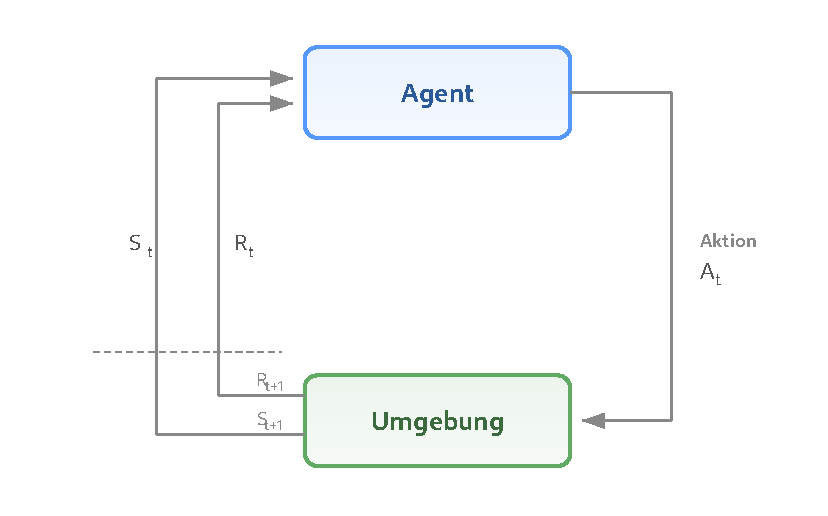
\includegraphics[width=0.65\linewidth]{Bilder/mdp_agent_environment.pdf}
    \caption{Interaktion zwischen Agent und Umgebung in einem MDP (nach \cite{suttonReinforcementLearningIntroduction2020}, S.~48).}
    \label{fig:mdp_agent_environment}
\end{figure}

Die Übergangsdynamik der Umgebung wird durch die Funktion
\begin{equation} \label{eq:mdp_dynamics}
    p(s', r \mid s, a) = \Pr\{S_{t+1} = s',\, R_{t+1} = r \mid S_t = s, A_t = a\}
\end{equation}
vollständig charakterisiert, welche die Wahrscheinlichkeit angibt, ausgehend vom Zustand $s$ bei gewählter Aktion $a$ in den Folgezustand $s'$ überzugehen und dabei die Belohnung $r$ zu erhalten. Wesentlich ist dabei die \Fachbegriff{Markov-Eigenschaft}: Folgezustand und Belohnung hängen ausschließlich vom gegenwärtigen Zustand-Aktions-Paar $(s,a)$ ab.

Das Ziel des Agenten besteht darin, durch Interaktion mit der Umgebung eine Strategie $\pi(a \mid s)$ zu identifizieren, welche die über die Zeit kumulierte Belohnung maximiert. Eine solche Strategie wird als \NeuerBegriff{optimale Strategie} bezeichnet und mit $\pi_*$ gekennzeichnet.



\section{Lösungen von MDPs}
\label{sec:ppo}

Welche Verfahren zur Bestimmung einer optimalen Strategie geeignet sind, hängt maßgeblich von der Formulierung des Reinforcement-Learning-Problems ab. Die klassische Theorie liefert exakte Lösungen ausschließlich für endliche MDPs mit vollständig bekanntem Übergangsmodell; ihre Grundideen lassen sich jedoch auf komplexere Problemklassen verallgemeinern.
Dieser Abschnitt behandelt die Lösung von MDPs. Eingeführt werden zunächst tabellarische Verfahren, anschließend Funktionsapproximation und schließlich Policy-Gradient-Methoden, die in das Verfahren der \Fachbegriff{Proximal Policy Optimization} (PPO) münden.

\subsection{Dynamische Programmierung}
\label{subsec:dp}

Das Ziel des Agenten besteht in der Maximierung des erwarteten Ertrags $G_t = \sum_{k=0}^{\infty} \gamma^k R_{t+k+1}$ mit Diskontierungsfaktor $\gamma \in [0,1)$. Die Güte einer Strategie $\pi$ wird durch die Zustandswertfunktion $v_\pi(s) = \mathbb{E}_\pi[G_t \mid S_t = s]$ charakterisiert, die den erwarteten Ertrag ausgehend von einem Zustand angibt. Die Zustandswertfunktion der optimalen Strategie $\pi_*$ wird als $v_*$ bezeichnet. Ihre direkte Berechnung setzt jedoch ein vollständig bekanntes Übergangsmodell und einen abzählbaren Zustandsraum voraus. In der Praxis sind beide Voraussetzungen selten gleichzeitig erfüllt: Das Übergangsmodell physikalischer Systeme ist in der Regel nicht vollständig bekannt, und selbst bei bekanntem Modell übersteigt der Zustandsraum realistischer Probleme typischerweise jene Dimensionen, in denen eine exakte Lösung mit vertretbarem Rechenaufwand möglich wäre.

\subsection{Monte-Carlo- und Temporal-Difference-Verfahren}
\label{subsec:mc_td}

Das fehlende Modell als erste Einschränkung wird durch \Fachbegriff{sample-basierte} Verfahren wie Monte-Carlo- und Temporal-Difference-Methoden (TD) aufgehoben. Monte-Carlo-Methoden benötigen den vollständigen Episodenertrag $G_t$ und können die Wertschätzung daher erst nach Abschluss einer Episode aktualisieren. TD-Verfahren hingegen nutzen \Fachbegriff{Bootstrapping} und korrigieren ihre Schätzung nach jedem einzelnen Zeitschritt anhand der geschätzten Bewertung des Folgezustands:
\begin{equation} \label{eq:td_update}
    V(S_t) \leftarrow V(S_t) + \alpha \bigl[R_{t+1} + \gamma\, V(S_{t+1}) - V(S_t)\bigr].
\end{equation}
TD-Verfahren bilden die Grundlage der meisten modernen Reinforcement-Learning-Algorithmen: Sie können online angewandt werden, benötigen wenig Rechenaufwand und lassen sich mit Funktionsapproximation auf große Zustandsräume skalieren.

\subsection{Funktionsapproximation}
\label{subsec:function_approximation}


Die Dimensionalität des Zustandsraums als zweite Einschränkung kann durch \NeuerBegriff{Funktionsapproximation} überwunden werden. Statt jeden Zustand mit einem eigenen Eintrag zu versehen, wird die Wertfunktion durch eine parametrisierte Funktion $\hat{v}(s, \mathbf{w})$ mit $\mathbf{w} \in \mathbb{R}^d$ und $d \ll |\mathcal{S}|$ dargestellt und in Richtung~$v_\pi$ optimiert.
Parametrisierte Funktionen erlauben Generalisierung: Erfahrungen, die über einen Zustand gemacht wurden, lassen sich auf benachbarte Zustände übertragen; gleichzeitig werden kontinuierliche Zustandsräume handhabbar. Als Parametrisierung eignen sich insbesondere neuronale Netze, da diese als universelle Funktionsapproximatoren in der Lage sind, beliebige stetige Funktionen auf kompakten Teilmengen beliebig genau anzunähern \autocite{hornikMultilayerFeedforwardNetworks1989}.

Während die Funktionsapproximation das Problem kontinuierlicher Zustandsräume löst, bleibt ein zweites Hindernis bei kontinuierlichen \emph{Aktionsräumen} bestehen. Wertbasierte Verfahren wählen Aktionen gemäß $a = \arg\max_{a'} \hat{q}(s, a', \mathbf{w})$; dieses Maximum ist in kontinuierlichen Aktionsräumen jedoch im Allgemeinen nicht effizient berechenbar.

\subsection{Policy-Gradient-Methoden}
\label{subsec:policy_gradient}

Eine Alternative ist, die Strategie nicht über eine Wert-Funktion abzuleiten, sondern direkt als parametrisierte Funktion $\pi(a \mid s, \boldsymbol{\theta})$ zu beschreiben und ihre Parameter $\boldsymbol{\theta}$ durch Gradientenaufstieg zu optimieren. Der entscheidende Vorteil für diese Arbeit: Policy-Gradient-Methoden können auf natürliche Weise kontinuierliche Aktionsräume handhaben, wie sie in der Drohnensteuerung auftreten.

In der Praxis wird der Policy-Gradient-Ansatz häufig als \Fachbegriff{Actor-Critic-Architektur} umgesetzt: Ein \Fachbegriff{Actor}-Netz repräsentiert die Strategie $\pi(\cdot \mid \cdot, \boldsymbol{\theta})$, ein \Fachbegriff{Critic}-Netz schätzt eine Wert-Funktion $\hat v(\cdot, \mathbf{w})$. Die Wertschätzung des Critics dient als Referenzniveau, das die Varianz der Gradientenschätzung reduziert, ohne sie zu verzerren.

\subsection{Proximal Policy Optimization}
\label{subsec:ppo_clip}

Eine moderne und in der Praxis weit verbreitete Variante des Policy-Gradient-Ansatzes ist \Fachbegriff{Proximal Policy Optimization} (PPO) \autocite{schulmanProximalPolicyOptimization2017}, ein Actor-Critic-Verfahren, das die Trainingsstabilität von Trust-Region-Methoden erreicht und dabei wesentlich einfacher zu implementieren ist.

Zu große Strategieänderungen pro Optimierungsschritt können Policy-Gradient-Verfahren
destabilisieren, da die gesammelten Trajektorien für die veränderte Strategie nicht mehr
repräsentativ sind \autocite{schulmanProximalPolicyOptimization2017}. Trust-Region-Methoden
wie TRPO \autocite{schulmanTrustRegionPolicy2015} begrenzen daher die KL-Divergenz
zwischen aufeinanderfolgenden Strategien, erfordern dafür jedoch Approximationen zweiter
Ordnung. PPO erzielt eine vergleichbare Stabilisierung allein durch eine geklippte
Zielfunktion:
\begin{equation} \label{eq:ppo_clip}
    L^{\mathrm{CLIP}}(\boldsymbol{\theta}) = \hat{\mathbb{E}}_t\!\left[
        \min\!\left(
            r_t(\boldsymbol{\theta})\,\hat{A}_t,\;
            \mathrm{clip}\!\left(r_t(\boldsymbol{\theta}),\, 1-\varepsilon,\,
            1+\varepsilon\right) \hat{A}_t
        \right)
    \right],
\end{equation}
wobei $r_t(\boldsymbol{\theta}) = \pi_{\boldsymbol{\theta}}(a_t \mid s_t)\,/\,
\pi_{\boldsymbol{\theta}_{\mathrm{alt}}}(a_t \mid s_t)$ das
Wahrscheinlichkeitsverhältnis zwischen neuer und alter Strategie ist, $\hat{A}_t$ der
Vorteilsschätzer und $\varepsilon$ die Clipping-Grenze.
Das Clipping bewirkt \emph{pessimistische} Updates: Verbessert eine Strategieänderung
das Objective, wird der Anreiz bei $r_t > 1 + \varepsilon$ gekappt; verschlechtert sie
es, greift die Minimumbildung und die Korrektur bleibt uneingeschränkt
(Abbildung~\ref{fig:ppo_clip}). So werden zu große Schritte in Richtung guter
Erfahrungen gebremst, während schlechte Aktionen voll korrigiert werden.

\begin{figure}[ht]
    \centering
    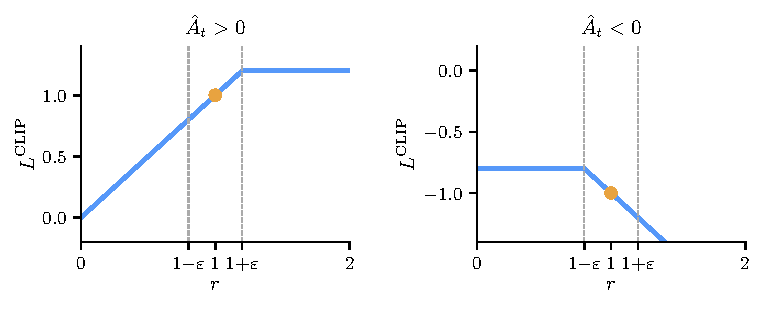
\includegraphics[width=0.85\linewidth]{Bilder/ppo_clipping.pdf}
    \caption{$L^{\mathrm{CLIP}}$ als Funktion des
    Wahrscheinlichkeitsverhältnisses~$r$. Links ($\hat{A}_t > 0$): der Anreiz wird bei
    $1 + \varepsilon$ gekappt. Rechts ($\hat{A}_t < 0$): die Korrektur bleibt
    uneingeschränkt (nach \autocite{schulmanProximalPolicyOptimization2017}, Fig.~1).}
    \label{fig:ppo_clip}
\end{figure}

Das vollständige PPO-Objective kombiniert das Clipping mit zwei weiteren Termen:
\begin{equation} \label{eq:ppo_full}
    L(\boldsymbol{\theta}) =
    L^{\mathrm{CLIP}}(\boldsymbol{\theta})
    - c_1\, L^{VF}(\boldsymbol{\theta})
    + c_2\, H\!\left[\pi_{\boldsymbol{\theta}}\right]\!(s_t),
\end{equation}
wobei $L^{VF} = (V_{\boldsymbol{\theta}}(s_t) - V_t^{\mathrm{targ}})^2$ der quadratische
Fehler der Wertfunktionsschätzung des Critics ist und
$H[\pi_{\boldsymbol{\theta}}]$ einen Entropie-Bonus bezeichnet, der vorzeitige
Konvergenz der Aktionsverteilung verhindert. Ohne diesen Term kann die
Standardabweichung gegen null konvergieren (\Fachbegriff{Std-Collapse}), was die Strategie
irreversibel auf eine deterministische Aktion festlegt.

Für die Schätzung des Vorteils~$\hat{A}_t$ wird \Fachbegriff{Generalized Advantage Estimation}
(GAE) \autocite{schulmanHighDimensionalContinuousControl2016} eingesetzt, das über den
Parameter~$\lambda$ einen Kompromiss zwischen Bias und Varianz der Vorteilsschätzung
steuert.

\section{Convolutional Neural Networks}
\label{sec:cnn}

\NeuerBegriff{Convolutional Neural Networks} (CNNs) sind eine Klasse neuronaler Netze, die speziell für die Verarbeitung von Daten mit räumlicher Struktur entwickelt wurden, etwa Bilder in Form zweidimensionaler Pixelarrays. Sofern nicht anders angegeben, folgt die Darstellung in diesem Abschnitt \textcite{lecunDeepLearning2015}.

Die Architektur eines CNN besteht aus einer Kaskade von Faltungs- und Pooling-Schichten. In einer \Fachbegriff{Faltungsschicht} sind die Einheiten in sogenannten \Fachbegriff{Feature Maps} organisiert. Jede Einheit ist nur mit einem lokalen Ausschnitt der vorherigen Schicht verbunden und verrechnet diesen mit einem \Fachbegriff{Filter} (auch \Fachbegriff{Kernel}), einer kleinen quadratischen Gewichtsmatrix \autocite{botschParametrischeMethoden2023}. Dabei werden die überdeckten Eingabewerte elementweise mit den Filtergewichten multipliziert und zu einem einzelnen Ausgabewert aufsummiert. Alle Einheiten innerhalb einer Feature Map teilen denselben Filter; mathematisch entspricht diese Operation einer diskreten Faltung. Verschiedene Feature Maps innerhalb einer Schicht verwenden unterschiedliche Filter und erkennen dadurch unterschiedliche lokale Muster. Die Filtergewichte werden nicht manuell festgelegt, sondern während des Trainings gelernt \autocite{botschParametrischeMethoden2023}. Die gemeinsame Nutzung der Gewichte beruht auf zwei Eigenschaften natürlicher Bilddaten: Benachbarte Werte bilden häufig korrelierte lokale Muster, und diese Muster treten unabhängig von ihrer Position im Bild auf.

\Fachbegriff{Pooling-Schichten} fassen die Aktivierungen benachbarter Einheiten zusammen, typischerweise durch Auswahl des Maximums innerhalb eines lokalen Fensters (\Fachbegriff{Max-Pooling}) \autocite{botschParametrischeMethoden2023}. Dies reduziert die räumliche Auflösung der Repräsentation und erzeugt eine gewisse Invarianz gegenüber kleinen Verschiebungen im Eingabebild.

Durch das Stapeln mehrerer Faltungs- und Pooling-Stufen entsteht eine hierarchische Merkmalsextraktion: Frühe Schichten erkennen einfache lokale Strukturen wie Kanten, mittlere Schichten kombinieren diese zu komplexeren Motiven, und tiefe Schichten repräsentieren ganze Objektteile. Die resultierende kompakte Repräsentation kann als Eingabe für nachgeschaltete Netzwerkkomponenten dienen. \textcite{mnihHumanlevelControlDeep2015} zeigten erstmals, dass ein CNN in dieser Rolle als Merkmalsextraktor innerhalb eines Reinforcement-Learning-Systems eingesetzt werden kann, indem sie eine Strategie direkt aus hochdimensionalen Bilddaten lernten.

\section{Achsenparallele Begrenzungsboxen}
\label{sec:aabb}

Eine \NeuerBegriff{achsenparallele Begrenzungsbox} (\Fachbegriff{Axis-Aligned Bounding Box}, AABB) ist das kleinste achsenparallele Quader, das ein gegebenes Objekt vollständig umschließt. Sie wird durch zwei Punkte definiert: das komponentenweise Minimum und Maximum aller Objektpunkte,
\begin{equation}
    \mathbf{p}_{\min} = \bigl(\min_i x_i,\, \min_i y_i,\, \min_i z_i\bigr), \quad
    \mathbf{p}_{\max} = \bigl(\max_i x_i,\, \max_i y_i,\, \max_i z_i\bigr),
\end{equation}
wobei $(x_i, y_i, z_i)$ die Eckpunkte bzw.\ Oberflächenpunkte des Objekts bezeichnen.

Die AABB besitzt eine \Fachbegriff{konservative} Eigenschaft: Da sie das Objekt vollständig umschließt, wird jede tatsächliche Kollision mit dem Objekt auch als Kollision mit der AABB erkannt. Im Umkehrschluss kann ein Punkt jedoch innerhalb der AABB liegen, ohne das eingeschlossene Objekt zu berühren. Der Approximationsfehler wächst mit der Abweichung der Objektgeometrie von einer quaderförmigen Gestalt; bei konkaven oder stark unregelmäßigen Formen kann die AABB ein erheblich größeres Volumen als das Objekt selbst einnehmen.

Für die Kollisionserkennung in Echtzeitsystemen bietet die AABB einen günstigen Kompromiss: Der Abstandstest reduziert sich auf sechs skalare Vergleiche pro Achse und ist damit wesentlich effizienter als Distanzberechnungen auf der tatsächlichen Objektgeometrie. Dem steht die beschriebene konservative Approximation gegenüber, die zu falsch-positiven Kollisionserkennungen führen kann.
\chapter{Stand der Forschung}
\label{cha:Stand der Forschung}

\section{Autonomes Landen von Drohnen}
\label{sec:landen}

Bisherige Arbeiten zum autonomen Landen von Drohnen lassen sich in zwei grundlegende Kategorien einteilen: traditionelle und bildbasierte Methoden.
Traditionelle Methoden stützen sich auf Signale externer Infrastruktur wie GNSS-Satelliten oder Funkbaken, um Position und Lage der Drohne zu bestimmen.
Bildbasierte Methoden hingegen nutzen Kameradaten zur Wahrnehmung der Umgebung und lassen sich weiter unterteilen in markerbasierte Systeme, die definierte
visuelle Referenzpunkte zur Lokalisierung verwenden, und markerfreie Systeme, die adäquate Landezonen eigenständig aus Bilddaten ableiten und somit keine
zusätzliche Bodeninfrastruktur erfordern. Diese Einteilung orientiert sich an der Taxonomie von \textcite{arafatVisionBasedNavigationTechniques2023}.

Orthogonal zur Sensorik lassen sich Ansätze danach unterscheiden, welche Teilaufgaben des Guidance, Navigation and Control (GNC) \autocite{kanellakisSurveyComputerVision2017} sie adressieren und wie diese zusammenwirken. Modulare Methoden zerlegen das Problem in getrennte Komponenten wie Obstacle Detection, Pose-Estimation oder Path-Planning, die als aufeinanderfolgende Stufen einer Pipeline gelöst werden \autocite{kanellakisSurveyComputerVision2017, wangVisionBasedDeepReinforcement2024}. End-to-End-Methoden hingegen bilden Sensorinput direkt auf Steuerkommandos ab, ohne solche expliziten Zwischenstufen \autocite{wangVisionBasedDeepReinforcement2024}.

GNSS ist die verbreitetste Methode zur Positionsbestimmung von Drohnen: Ein einzelnes GNSS-Modul liefert eine Genauigkeit von 5–10\,m und bildet die Grundlage für Missionsplanung und -ausführung \autocite{jarrayaGnssdeniedUnmannedAerial2025}. Dass autonomes Landen bei bekannter Relativposition grundsätzlich beherrschbar ist, zeigen \textcite{voosNonlinearTrackingLanding2010} mittels nichtlinearer Regelung auf stationären und beweglichen Zielen. Die zentrale Herausforderung liegt somit nicht im Regelungsentwurf, sondern in der Genauigkeit der zugrunde liegenden Positionsdaten.

In der Praxis erreicht GNSS-basierte Landung jedoch nur Meter-Genauigkeit. \textcite{patrikGNSSbasedNavigationSystems2019} berichten von einer durchschnittlichen Landeabweichung von 1,11\,m; auch beim Open-Source-Autopiloten PX4 beträgt die GNSS-basierte Landegenauigkeit mehrere Meter \autocite{meierPX4NodebasedMultithreaded2015, wubbenAccurateLandingUnmanned2019}, sodass für höhere Präzision zusätzliche Sensoren erforderlich sind \autocite{PrecisionLanding}. Die Positionsgenauigkeit lässt sich zwar durch RTK-Korrekturen auf Zentimeter-Niveau steigern — \textcite{tavasciReliabilityRealTimeKinematic2024} berichten zentimetergenaue Echtzeit-Navigation unter idealen Bedingungen —, allerdings fällt die Genauigkeit in schwierigen GNSS-Umgebungen, etwa bei Signalabschattung durch Vegetation oder Gebäude, auf Meter-Niveau zurück. Gerade in Agrarumgebungen mit Baumkronen und Laubdächern sind solche Bedingungen typisch.

GNSS bleibt damit als robuste Grobpositionierung unverzichtbar, weist jedoch für Präzisionslandung in strukturierten Umgebungen fundamentale Limitationen auf: Die Genauigkeit reicht nicht für das Landen zwischen Baumreihen oder Weinreben mit einem typischen Reihenabstand von 1,5–2\,m. Zudem liefert GNSS keinerlei Umgebungswahrnehmung; Veränderungen der Umgebung, Hindernisse oder beengte Platzverhältnisse bleiben unerkannt.

Bildbasierte Landesysteme mit visuellen Markern bieten eine deutlich höhere Präzision als rein GNSS-gestützte Methoden. So erreicht das ArUco-basierte System von \textcite{wubbenAccurateLandingUnmanned2019} durch deterministische Bildverarbeitung eine durchschnittliche Landeabweichung von 11\,cm bei zuverlässiger Markerdetektion aus bis zu 30\,m Höhe. Solche klassischen Ansätze setzen jedoch voraus, dass die Markererkennung unter allen Betriebsbedingungen robust funktioniert — eine Annahme, die bei Verdeckung, wechselnden Lichtverhältnissen oder beschädigten Markern nicht gegeben ist.

Reinforcement Learning bietet hier einen konzeptionellen Vorteil: Statt auf handspezifizierte Detektionsalgorithmen angewiesen zu sein, lernt ein RL-Agent eine End-to-End-Steuerung direkt aus Bilddaten und kann dabei implizit Robustheit gegenüber visuellen Störungen erwerben. \textcite{polvaraSimtoRealQuadrotorLanding2020} demonstrieren diesen Ansatz erstmals für die autonome Landung: Ihr System nutzt sequentielle Deep-Q-Networks mit diskretem Aktionsraum und einer Divide-and-Conquer-Strategie, die den Landeprozess in Marker-Ausrichtung und vertikalen Abstieg unterteilt — ein Ansatz, der das Problem dünn besetzter Belohnungssignale adressiert, indem die komplexe Aufgabe in einfachere Teilziele zerlegt wird. Als einziger Sensor dient eine niedrig aufgelöste monokulare Graustufenkamera. Ausschließlich in Simulation mit Domain Randomization trainiert, erzielt das System Erfolgsraten von 89\,\% für den vertikalen Abstieg, die im realen Flug auf 61\,\% sinken. Der Robustheitsvorteil gegenüber klassischen Methoden zeigt sich unter erschwerten Bedingungen: Bei verrauschten Markertexturen erreicht das RL-System noch 51\,\%, während ein konventioneller AR-Tracker vollständig versagt — allerdings ist auch dieser Wert für sicherheitskritische Anwendungen unzureichend. Eine zentrale methodische Einschränkung bleibt der diskrete Aktionsraum, der die Steuerungspräzision limitiert.

\textcite{ladoszAutonomousLandingMoving2024} erweitern den Ansatz auf bewegliche Landeplattformen und adressieren diese Einschränkung durch einen kontinuierlichen Aktionsraum, der erstmals auch die Vertikalgeschwindigkeit einschließt — bei früheren Arbeiten wird der vertikale Abstieg typischerweise regelbasiert gesteuert. Der Agent erhält neben Graustufenbildern auch IMU-Daten (Geschwindigkeit und Lage) als Zustandsinformation. In der Simulation erreicht das System Erfolgsraten von bis zu 97,4\,\% bei einer Landeabweichung von 0,52\,m; im realen Transfer sinkt die Rate auf rund 70\,\%. Die Autoren zeigen zudem, dass Domain Randomization zwar notwendig für den Sim-to-Real-Transfer ist, eine zu starke Randomisierung die Performance jedoch signifikant verschlechtert. Die Experimente beschränken sich auf einfache Szenarien ohne Hindernisse und gleichmäßig beleuchtete Innenräume.

Trotz dieser Fortschritte weisen markerbasierte Systeme grundlegende Einschränkungen auf, die unabhängig von der gewählten Steuerungsmethode gelten: Sie setzen vorplatzierte visuelle Infrastruktur am Landeziel voraus, was ihren Einsatz auf vordefinierte Orte begrenzt und in unbekannten Umgebungen unpraktikabel macht. Hinzu kommen methodische Limitationen der RL-basierten Ansätze: Beide Systeme wurden in vereinfachten Simulationsumgebungen ohne Hindernisse trainiert, und der Transfer in die reale Welt geht mit deutlichen Leistungseinbußen einher — \textcite{ladoszAutonomousLandingMoving2024} berichten einen Rückgang der Erfolgsrate von 97,4\,\% auf rund 70\,\% \autocite[vgl. auch][]{polvaraSimtoRealQuadrotorLanding2020}. Diese Limitationen motivieren die Entwicklung markerfreier Systeme, die Landezonen eigenständig aus Bilddaten ableiten und keine zusätzliche Bodeninfrastruktur erfordern.

Markerfreie Verfahren ermöglichen den Einsatz in unbekannten, unstrukturierten und dynamischen Umgebungen, da sie keine manuelle Vorbereitung der Landezone erfordern — eine Eigenschaft, die insbesondere für Notlandungen oder den Betrieb in unzugänglichen Gebieten entscheidend ist \autocite{yangMonocularVisionSLAMBased2018, bartolomeiAutonomousEmergencyLanding2022}. Die Bandbreite der Ansätze reicht dabei von klassischen modularen Pipelines bis hin zu End-to-End-Steuerungen mittels Deep Reinforcement Learning.

\textcite{yangMonocularVisionSLAMBased2018} verfolgen einen modularen Ansatz, bei dem aus monokularer SLAM-Rekonstruktion eine 3D-Punktwolke erzeugt wird, aus der anhand von Oberflächensemantik und Geländehöhe sichere Landezonen in einer Grid-Map identifiziert werden. Das System nutzt ausschließlich Visual-Inertial-Odometrie zur Zustandsschätzung und benötigt weder GNSS noch externe Lokalisierungsinfrastruktur. Es demonstriert Landungen in verschiedenen Umgebungen, weist jedoch aufgrund der hohen Pipeline-Komplexität eine Landezeit von rund zwei Minuten auf.

Einen End-to-End-Ansatz wählen \textcite{bartolomeiAutonomousEmergencyLanding2022}: Ihr RL-Agent bildet Tiefenbilder und semantische Segmentierungen — sogenannte Mid-Level-Repräsentationen, die generischer als Rohbilder sind und schnelleres Training ermöglichen — direkt auf diskrete Steuerkommandos ab. Das System erreicht in der Simulation Erfolgsraten von über 70\,\% bei minimaler Sensorausstattung mit lediglich einer monokularen RGB-Kamera. Ein methodisch relevanter Aspekt ist die Sim-to-Real-Strategie: Die Policy wird zunächst mit Ground-Truth-Tiefen- und Semantikdaten trainiert und anschließend mit verrauschten Prädiktionen neuronaler Netze feinabgestimmt, um den Simulationstransfer zu ermöglichen. Im Realflug landete die Policy erfolgreich, während sowohl eine kommerzielle als auch eine State-of-the-Art-Lösung am verrauschten Sensorinput scheiterten. Einschränkend setzt das System voraus, dass semantische Segmentierungen und Tiefenbilder stets verfügbar sind, und der diskrete Aktionsraum (zehn mögliche Aktionen) limitiert die Steuerungsflexibilität.

Dass Deep Reinforcement Learning auch unter dynamischen Umgebungsbedingungen effektive Landesteuerungen ermöglicht, zeigen \textcite{peterTornadoDroneBioinspiredDRLbased2024} mit TornadoDrone: Das bio-inspirierte DRL-Framework übertrifft eine konventionelle PID+EKF-Baseline bei Landungen unter starken Windturbulenzen deutlich, stützt sich in den realen Experimenten jedoch auf ein Vicon-Lokalisierungssystem, das unter Einsatzbedingungen nicht verfügbar ist.

\section{Tiefenbildbasierte Hindernisvermeidung}
\label{sec:tiefenbild-oa}

\textcite{loquercioLearningHighspeedFlight2021} demonstrieren ein End-to-End-Navigationssystem für Hochgeschwindigkeitsflüge durch komplexe, unbekannte Umgebungen mit ausschließlich bordeigener Sensorik und Rechenleistung. Das System nutzt Tiefenbilder einer Stereokamera und IMU-Daten, um kollisionsfreie Kurzzeittrajektorien zu erzeugen, die von einem nachgeschalteten PID-Regler ausgeführt werden. Trainiert wird ausschließlich in Simulation mittels Privileged Learning, einer Imitation eines Experten mit Zugang zu perfekter Zustandsinformation, wobei lediglich einfache Hindernisgeometrien (Zylinder, Quader, Baumstämme) verwendet werden. Durch die Simulation realistischen Sensorrauschens gelingt ein Zero-Shot-Transfer in reale Umgebungen, die während des Trainings nie erfahren wurden: dichte Wälder, verschneites Gelände und eingestürzte Gebäude. Bei niedrigen Geschwindigkeiten erreicht das System eine Erfolgsrate von 100\,\% in allen getesteten Umgebungen; im Vergleich zu modularen State-of-the-Art-Planern reduziert der Ansatz die Ausfallrate um den Faktor~10. Eine Einschränkung ist die geringe Positioniergenauigkeit, da Erfolg bereits bei einem Abstand von 5\,m zum Ziel definiert wird und der Fokus auf Geschwindigkeit statt Präzision liegt. Methodisch relevant für die vorliegende Arbeit ist der Nachweis, dass ein lernbasierter Ansatz mit Tiefenbildern und hierarchischer Architektur (Policy $\rightarrow$ PID) in dicht bewachsenen natürlichen Umgebungen robust navigieren kann. Die vorliegende Arbeit verfolgt eine vergleichbare Architektur, ersetzt jedoch Privileged Learning durch Reinforcement Learning und verschiebt den Fokus von Hochgeschwindigkeitsnavigation auf Präzisionslandung in beengten Umgebungen.

\textcite{kimMonocularVisionbasedAutonomous2022} verfolgen einen zweistufigen Ansatz, bei dem zunächst ein vortrainiertes CNN Tiefenbilder aus monokularen RGB-Aufnahmen schätzt und anschließend ein Dueling-Double-DQN auf Basis dieser geschätzten Tiefeninformation diskrete Ausweichentscheidungen trifft. Als einziger externer Sensor dient die bordeigene Monokularkamera der Drohne; Zustandsinformation wie Position oder Geschwindigkeit wird nicht benötigt. Das System wird in Simulation trainiert und ohne weitere Anpassung auf eine reale Drohne übertragen, wo es enge Korridore mit texturlosen Wänden, Personen und Kisten kollisionsfrei durchfliegt. Evaluiert wird anhand der zurückgelegten Strecke ohne Kollision; eine gezielte Navigation zu einem definierten Ziel ist nicht Teil des Systems. Die Testumgebungen beschränken sich auf strukturierte Innenräume; Experimente in natürlichen oder vegetationsreichen Umgebungen werden nicht durchgeführt. Der Ansatz demonstriert, dass selbst aus monokularer RGB-Eingabe geschätzte Tiefeninformation für lernbasierte Hindernisvermeidung ausreicht, allerdings mit den Einschränkungen eines diskreten Aktionsraums und der Abhängigkeit von der Qualität der Tiefenschätzung.

\textcite{xuNavRLLearningSafe2024} nutzen direkte Tiefenbilder, um mittels PPO eine kontinuierliche Policy für sichere Navigation in Umgebungen mit statischen und dynamischen Hindernissen zu trainieren. Die Architektur verarbeitet die Tiefenbilder zu einer 3D-Belegungskarte, die zusammen mit Drohnenzustandsdaten (Position, Geschwindigkeit, Orientierung) als Eingabe für das Actor-Critic-Netzwerk dient. Das Training erfolgt parallelisiert in Simulation mit Curriculum Learning, bei dem die Anzahl dynamischer Hindernisse schrittweise erhöht wird. Ein nachgeschalteter Safety Shield auf Basis von Velocity Obstacles ergänzt die gelernte Policy zur Laufzeit. Das System erreicht Zero-Shot-Transfer auf eine reale Drohne und erzielt in Szenarien mit dynamischen Hindernissen die geringste Kollisionsrate im Vergleich zu bestehenden Methoden. Auch hier beschränken sich die Testumgebungen auf strukturierte Indoor-Szenarien mit geometrisch einfachen Hindernissen.

Gemeinsam zeigen diese Arbeiten, dass tiefenbildbasierte lernende Systeme Hindernisse zuverlässig vermeiden können, unabhängig davon ob die Tiefeninformation direkt gemessen \autocite{loquercioLearningHighspeedFlight2021, xuNavRLLearningSafe2024} oder aus RGB-Bildern geschätzt wird \autocite{kimMonocularVisionbasedAutonomous2022}. Allerdings testen alle genannten Systeme in strukturierten Innenräumen oder Waldumgebungen; Evaluationen in landwirtschaftlichen Umgebungen mit Rebzeilen, niedrigen Baumkronen oder dichter Bodenvegetation fehlen.

Vereinzelte Arbeiten adressieren die Navigation in landwirtschaftlichen Umgebungen gezielt. \textcite{weiVisionBasedNavigation2025} demonstrieren ein lernbasiertes UAV-System für die autonome Navigation durch Obstplantagen-Reihen: Ein VAE-Controller, trainiert mittels Imitation Learning aus Expertendemonstrationen, steuert einen Quadrotor auf Basis einer front-montierten RGB-Kamera kollisionsfrei zwischen Baumreihen. Das System generalisiert auf ungesehene Umgebungen und kommt ohne GPS aus, beschränkt sich jedoch auf horizontale Reihennavigation. Für Weinberge zeigen \textcite{martiniPositionAgnosticAutonomous2022}, dass ein DRL-Agent auf Basis von Tiefenbildern ohne Positionsinformation durch simulierte Rebzeilen navigieren kann, allerdings mit einem Bodenroboter statt einer Drohne. Beide Arbeiten bestätigen, dass Vegetation in landwirtschaftlichen Umgebungen eine eigenständige Navigationsherausforderung darstellt, die durch lernbasierte Ansätze mit minimaler Sensorik adressiert werden kann. Keine der Arbeiten behandelt jedoch die vertikale Landung zwischen Vegetationsstrukturen, die eine kombinierte Hindernisvermeidung und Präzisionspositionierung erfordert.

\section{Reinforcement Learning für Drohnensteuerung}
\label{sec:architektur}

Über die Wahl der Sensorik hinaus beeinflusst die Steuerungsarchitektur die Leistungsfähigkeit lernbasierter Drohnensysteme maßgeblich, insbesondere der Aktionsraum und die Abstraktionsebene der Regelung. Die in den Abschnitten~\ref{sec:landen} und~\ref{sec:tiefenbild-oa} betrachteten Arbeiten lassen sich auch entlang dieser Dimension einordnen: End-to-End-Systeme wie \autocite{polvaraSimtoRealQuadrotorLanding2020, kimMonocularVisionbasedAutonomous2022, ladoszAutonomousLandingMoving2024} erzeugen Bewegungskommandos direkt aus Sensorinput, während hierarchische Ansätze wie \autocite{loquercioLearningHighspeedFlight2021, bartolomeiAutonomousEmergencyLanding2022} die Policy-Ausgabe an einen nachgeschalteten Regler delegieren. \textcite{xuNavRLLearningSafe2024} kombinieren beide Paradigmen, indem sie eine PPO-Policy mit einem regelbasierten Safety Shield ergänzen.

Die Wahl der Abstraktionsebene beeinflusst die Lernperformance substanziell: \textcite{esserActionSpaceDesign2024} zeigen in einer systematischen Studie über verschiedene Roboterplattformen und Aufgaben, dass der optimale Aktionsraum stark aufgabenabhängig ist und unterschiedliche Abstraktionsebenen zu deutlich verschiedenem Explorationsverhalten und finaler Performance führen. Speziell für Quadrotoren vergleichen \textcite{kaufmannBenchmarkComparisonLearned2022} drei Abstraktionsebenen: Geschwindigkeitskommandos, kollektiven Schub mit Drehraten sowie direkte Einzelmotorschübe. Die mittlere Ebene (Schub und Drehraten) erweist sich als beste Balance zwischen Agilität und Transferrobustheit; die höchste Abstraktion (Geschwindigkeit) schränkt die Manövrierfähigkeit ein, während die niedrigste (Einzelmotorschub) zu latenzempfindlich für den Realtransfer ist.

Neben der Steuerungsarchitektur hat sich PPO als verbreiteter Trainingsalgorithmus für RL-basierte Drohnensteuerung etabliert. Als Policy-Gradient-Verfahren eignet sich PPO für die kontinuierlichen Aktionsräume der Drohnensteuerung (vgl.\ Abschnitt~\ref{subsec:ppo_clip}). Da Reinforcement Learning grundsätzlich große Datenmengen benötigt, hat sich GPU-parallele Simulation als effektiver Ansatz etabliert: \textcite{rudinLearningWalkMinutes2022} zeigen, dass massiv-parallele Simulation mit hunderten bis tausenden Umgebungsinstanzen die Trainingszeit drastisch reduziert und schnellere Konvergenz ermöglicht. PPO eignet sich als On-Policy-Verfahren für dieses Paradigma, da es die parallel erzeugten Daten direkt verarbeitet und keinen Replay Buffer benötigt. Obwohl Off-Policy-Verfahren wie SAC eine höhere Sample-Effizienz bieten, zeigen \textcite{tayarAutonomousUAVFlight2025}, dass PPO bei sicherheitskritischen Präzisionsaufgaben in beengten Räumen zuverlässiger konvergiert als SAC. In den in diesem Kapitel betrachteten Arbeiten setzen \textcite{bartolomeiAutonomousEmergencyLanding2022}, \textcite{xuNavRLLearningSafe2024} und \textcite{kaufmannBenchmarkComparisonLearned2022} PPO ein; \textcite{kaufmannChampionlevelDroneRacing2023} demonstrieren den bislang eindrucksvollsten Einsatz, bei dem ein ausschließlich in Simulation trainiertes System drei menschliche Weltmeister im physischen Drohnenrennen schlägt.

Die vorliegende Arbeit folgt dem hierarchischen Paradigma und wählt eine noch höhere Abstraktionsebene als die von \textcite{kaufmannBenchmarkComparisonLearned2022} untersuchten: Der RL-Agent gibt eine Zielposition vor, die ein kaskadierender PID-Regler (Position $\rightarrow$ Geschwindigkeit $\rightarrow$ Lage $\rightarrow$ Drehzahl) in Motorkommandos umsetzt. Diese Wahl opfert bewusst Agilität zugunsten reduzierter Lernkomplexität, da die Aufgabe Präzisionslandung statt agilen Flugs erfordert. Die Ausgabe des Agenten bleibt interpretierbar, der PID-Regler kann unabhängig vom RL-Training auf die Zielplattform abgestimmt werden, und die Lernkomplexität reduziert sich auf die Frage, \emph{wohin} die Drohne fliegen soll.

Die Wahl der Sensorausstattung ist ein weiterer zentraler Designparameter: Drohnen sind aufgrund ihrer Energie- und Gewichtsbeschränkungen typischerweise nur mit minimaler Sensorik ausgestattet, bestehend aus Kameras und Distanzsensoren \autocite{bartolomeiAutonomousEmergencyLanding2022}. \textcite{semerikovVisionBasedAutonomousUAV2025} zeigen in ihrer Übersichtsarbeit, dass Vision-Inertial-Kombinationen eine gute Balance zwischen Wahrnehmungsleistung und Systemkomplexität bieten, während leistungsfähigere Sensorsetups entsprechend größere Drohnen mit höherer Lade- und Batteriekapazität erfordern. Gleichzeitig ermöglichen moderne Algorithmen, insbesondere lernbasierte Ansätze, dass auch mit leichtgewichtiger Sensorik anspruchsvolle Aufgaben gelöst werden können, die bisher komplexere Hardware voraussetzten. Die in diesem Kapitel betrachteten Arbeiten bestätigen diesen Trend: Erfolgreiche Hindernisvermeidung und Navigation gelingen mit einer einzelnen Kamera \autocite{kimMonocularVisionbasedAutonomous2022, polvaraSimtoRealQuadrotorLanding2020, bartolomeiAutonomousEmergencyLanding2022} oder einer Tiefenkamera mit IMU-Zustandsdaten \autocite{loquercioLearningHighspeedFlight2021, xuNavRLLearningSafe2024}. Die vorliegende Arbeit folgt diesem Prinzip minimaler Sensorik: Als Eingabe dienen eine nach unten gerichtete Tiefenkamera und ein Zustandsvektor (Position, Orientierung, Geschwindigkeit), wobei die algorithmische Komplexität des RL-Agenten die begrenzte Sensorausstattung kompensiert.

Tabelle~\ref{tab:vergleich-sdf} stellt die in diesem Kapitel betrachteten Arbeiten anhand ihrer Kernmerkmale gegenüber.

\begin{table}[htbp]
\centering
\caption{Vergleich der betrachteten Arbeiten zur autonomen Drohnennavigation und -landung. \emph{Hind.}: aktive Hindernisvermeidung; \emph{Landung}: Präzisionslandung als Teil der Aufgabe.}
\label{tab:vergleich-sdf}
\footnotesize
\setlength{\tabcolsep}{4pt}
\begin{tabular}{@{}lllcccc@{}}
\toprule
Arbeit & Sensorik & Methode & Akt.-raum & Hind. & Umgebung & Landung \\
\midrule
\textcite{polvaraSimtoRealQuadrotorLanding2020} & Mono RGB & DQN & diskret & -- & Indoor & $\checkmark$ \\
\textcite{ladoszAutonomousLandingMoving2024} & Mono RGB, IMU & DrQv2 & kont. & -- & Indoor & $\checkmark$ \\
\textcite{yangMonocularVisionSLAMBased2018} & Mono RGB & SLAM & -- & $\checkmark$ & Outdoor & $\checkmark$ \\
\textcite{bartolomeiAutonomousEmergencyLanding2022} & Mono RGB\textsuperscript{a} & PPO & diskret & $\checkmark$ & Outdoor & $\checkmark$ \\
\textcite{peterTornadoDroneBioinspiredDRLbased2024} & Vicon, IMU & TD3 & kont. & -- & Indoor & $\checkmark$ \\
\addlinespace
\textcite{loquercioLearningHighspeedFlight2021} & Stereo Tiefe, IMU & IL & kont. & $\checkmark$ & Outdoor & -- \\
\textcite{kimMonocularVisionbasedAutonomous2022} & Mono RGB\textsuperscript{b} & DQN & diskret & $\checkmark$ & Indoor & -- \\
\textcite{xuNavRLLearningSafe2024} & Tiefe, Zustand & PPO & kont. & $\checkmark$ & Indoor & -- \\
\textcite{weiVisionBasedNavigation2025} & Mono RGB & IL & kont. & $\checkmark$ & Agrar & -- \\
\textcite{martiniPositionAgnosticAutonomous2022}\textsuperscript{c} & Tiefe & SAC & kont. & $\checkmark$ & Agrar & -- \\
\addlinespace
Eigene Arbeit & Tiefe, Zustand & PPO & kont. & $\checkmark$ & Agrar & $\checkmark$ \\
\bottomrule
\end{tabular}

\smallskip
{\scriptsize
\textsuperscript{a} Eingabe: abgeleitete Tiefen- und Segmentierungsbilder. \quad
\textsuperscript{b} Eingabe: aus RGB geschätzte Tiefenbilder. \quad
\textsuperscript{c} Bodenroboter (UGV).
}
\end{table}

Zusammenfassend zeigt der Stand der Forschung drei wiederkehrende Limitationen RL-basierter Landesysteme: Erstens operieren die meisten Ansätze mit diskreten Aktionsräumen \autocite{polvaraSimtoRealQuadrotorLanding2020, bartolomeiAutonomousEmergencyLanding2022} oder vereinfachen den vertikalen Abstieg auf regelbasierte Steuerung — lediglich \textcite{ladoszAutonomousLandingMoving2024} setzen einen kontinuierlichen Aktionsraum mit Vertikalkontrolle ein, beschränken sich jedoch auf hindernisfreie Innenräume. Zweitens werden Hindernisvermeidung und Präzisionslandung überwiegend getrennt adressiert (vgl.\ Tabelle~\ref{tab:vergleich-sdf}): Systeme zur Hindernisvermeidung navigieren durch komplexe Umgebungen, ohne gezielt zu landen \autocite{loquercioLearningHighspeedFlight2021, kimMonocularVisionbasedAutonomous2022, xuNavRLLearningSafe2024}, während Landesysteme in der Regel in hindernisfreien Szenarien operieren \autocite{polvaraSimtoRealQuadrotorLanding2020, ladoszAutonomousLandingMoving2024}. Drittens bleibt der Sim-to-Real-Transfer eine offene Herausforderung: Die Erfolgsraten sinken systematisch beim Übergang in die reale Welt — von 89\,\% auf 61\,\% \autocite{polvaraSimtoRealQuadrotorLanding2020}, von 97,4\,\% auf rund 70\,\% \autocite{ladoszAutonomousLandingMoving2024} —, und reale Experimente stützen sich auf Hilfsmittel wie Vicon-Lokalisierung \autocite{peterTornadoDroneBioinspiredDRLbased2024} oder gezieltes Fine-Tuning \autocite{bartolomeiAutonomousEmergencyLanding2022}, die unter Einsatzbedingungen nicht verfügbar sind.

Die vorliegende Arbeit adressiert die ersten beiden Limitationen: Sie untersucht, ob ein RL-Agent mit kontinuierlichem Aktionsraum und Tiefenbildern in Simulation lernen kann, in beengten Umgebungen mit Hindernissen autonom zu landen. Ein vollständiger Sim-to-Real-Transfer liegt außerhalb des Rahmens dieser Arbeit. Um die Transferfähigkeit der gelernten Strategie dennoch zu untersuchen, wird ein Zero-Shot-Transfer in eine geometrisch verschiedenartige Simulationsumgebung (Sim-to-Sim) als vereinfachte Annäherung an die dritte Limitation eingesetzt.

\chapter{Methodik}
\label{cha:Methodik}

\section{Formulierung als Markov-Entscheidungsprozess}
\label{sec:meth_mdp}

Die autonome Drohnenlandung in einem vertikalen Korridor mit Hindernissen wird
als endlicher, episodischer Markov-Entscheidungsprozess (MDP) formalisiert
(vgl.\ Abschnitt~\ref{subsec:mdp}). Das MDP ist durch das Tupel
$(\mathcal{S}, \mathcal{A}, p, r, \gamma)$ definiert, wobei $\mathcal{S}$ den
Zustandsraum, $\mathcal{A}$ den Aktionsraum, $p$ die Übergangsdynamik, $r$ die
Belohnungsfunktion und $\gamma = 0{,}99$ den Diskontierungsfaktor bezeichnen.

\subsection{Zustandsraum}
\label{subsec:meth_zustandsraum}

Der Zustand $s_t \in \mathcal{S}$ zum Entscheidungszeitpunkt~$t$ setzt sich aus
einem numerischen Zustandsvektor $\mathbf{o}_t \in \mathbb{R}^{17}$ und einem
Tiefenbild $\mathbf{D}_t \in [0,1]^{64 \times 64}$ zusammen:
\begin{equation} \label{eq:meth_state}
  s_t = \bigl(\mathbf{o}_t,\;\mathbf{D}_t\bigr).
\end{equation}

Der Zustandsvektor
\begin{equation} \label{eq:meth_obs_vector}
  \mathbf{o}_t = \bigl(\,\tilde{\mathbf{p}}_{\mathrm{rel},t},\;\;
  \mathbf{q}_t,\;\;
  \tilde{\mathbf{v}}_t^{\,B},\;\;
  \tilde{\boldsymbol{\omega}}_t^{\,B},\;\;
  \mathbf{a}_{t-1}\,\bigr)
\end{equation}
enthält die in Tabelle~\ref{tab:meth_obs} aufgeschlüsselten Größen. Die Tilde
kennzeichnet skalierte und auf $[-1,1]$ geklippte Werte; die
Skalierungsfaktoren normieren die physikalischen Bereiche auf eine einheitliche
Größenordnung.

\begin{table}[ht]
\centering
\caption{Komponenten des Zustandsvektors $\mathbf{o}_t \in \mathbb{R}^{17}$.}
\label{tab:meth_obs}
\small
\begin{tabular}{l c l c}
\toprule
\textbf{Größe} & \textbf{Dim.} & \textbf{Beschreibung} & \textbf{Skalierung} \\
\midrule
$\tilde{\mathbf{p}}_{\mathrm{rel},t}$ & $3$ & Relative Position zum Ziel
  & $\times\tfrac{1}{15}$, ${\in}\,[-1,1]$ \\[2pt]
$\mathbf{q}_t$ & $4$ & Orientierungsquaternion $(w,x,y,z)$ & --- \\[2pt]
$\tilde{\mathbf{v}}_t^{\,B}$ & $3$ & Lineargeschwindigkeit
  & $\times\,0{,}4$, ${\in}\,[-1,1]$ \\[2pt]
$\tilde{\boldsymbol{\omega}}_t^{\,B}$ & $3$ & Winkelgeschwindigkeit
  & $\times\tfrac{1}{\pi}$, ${\in}\,[-1,1]$ \\[2pt]
$\mathbf{a}_{t-1}$ & $4$ & Aktion des vorherigen Zeitschritts & --- \\
\bottomrule
\end{tabular}
\end{table}

Die relative Position
$\tilde{\mathbf{p}}_{\mathrm{rel},t} =
\min\!\bigl(\max\!\bigl(\tfrac{1}{15}(\mathbf{p}_{\mathrm{ziel}} -
\mathbf{p}_t),\; -1\bigr),\; 1\bigr)$
kodiert Abstand und Richtung zum Landeziel, wobei der Skalierungsfaktor auf die
maximale Diagonaldistanz zum Ziel ausgelegt ist. Die Lineargeschwindigkeit wird
mit dem Faktor~$0{,}4$ skaliert, sodass der typische Geschwindigkeitsbereich der
Drohne auf $[-1,1]$ abgebildet wird; die Winkelgeschwindigkeit wird durch~$\pi$
dividiert und erreicht damit bei einer vollen Drehung pro Sekunde den
Sättigungswert.

Das Tiefenbild $\mathbf{D}_t \in [0,1]^{64 \times 64}$ wird von einer am
Drohnenkörper vertikal nach unten gerichteten Kamera mit $90^{\circ}$~Sichtfeld
erzeugt:
\begin{equation} \label{eq:meth_depth}
  \mathbf{D}_t = \min\!\left(\max\!\left(\frac{\mathbf{d}_{\mathrm{roh}}}{d_{\max}},
  \; 0\right),\; 1\right), \quad d_{\max} = 20\,\text{m}.
\end{equation}
Das Tiefenbild liefert die einzige Information über Lage und Geometrie der
Hindernisse; der numerische Zustandsvektor enthält keine explizite
Hindernisrepräsentation.

\subsection{Aktionsraum}
\label{subsec:meth_aktionsraum}

Der Aktionsraum ist vierdimensional und kontinuierlich:
\begin{equation} \label{eq:meth_action}
  \mathbf{a}_t = (a_x,\; a_y,\; a_z,\; a_\psi) \in [-1,\; 1]^4.
\end{equation}
Die ersten drei Komponenten definieren einen Positionsversatz relativ zur aktuellen
Drohnenposition:
\begin{equation} \label{eq:meth_target_pos}
  \mathbf{p}_{\mathrm{soll}} = \mathbf{p}_t +
  \begin{pmatrix} a_x \cdot \sigma_x \\ a_y \cdot \sigma_y \\ a_z \cdot \sigma_z \end{pmatrix},
  \quad \boldsymbol{\sigma} = (1{,}0;\; 1{,}0;\; 2{,}0)\,\text{m}.
\end{equation}
Die erhöhte $z$-Skala ermöglicht größere vertikale Schritte, die für den
vorwiegend vertikalen Abstieg erforderlich sind. Die vierte Komponente legt den
Sollgierwinkel fest:
\begin{equation} \label{eq:meth_target_yaw}
  \psi_{\mathrm{soll}} = a_\psi \cdot 180^{\circ}.
\end{equation}

Die Sollwerte $(\mathbf{p}_{\mathrm{soll}}, \psi_{\mathrm{soll}})$ werden
nicht direkt an die Motoren übergeben, sondern von einem kaskadierenden
PID-Regler in Motordrehzahlen umgesetzt
(vgl.\ Abschnitt~\ref{subsec:meth_uebergangsmodell}). Diese Entkopplung
reduziert den Aktionsraum von vier Motordrehzahlen auf vier semantisch
interpretierbare Navigationskommandos.

\subsection{Übergangsmodell}
\label{subsec:meth_uebergangsmodell}

Die Übergangsdynamik $p(s_{t+1} \mid s_t, \mathbf{a}_t)$ wird deterministisch
durch den Physiksimulator bestimmt. Der Simulator integriert die Physik mit
einer Schrittweite von $\Delta t = 0{,}01$\,s (100\,Hz). Der RL-Agent trifft
nicht bei jedem Simulationsschritt eine Entscheidung, sondern alle
300~Schritte, entsprechend einem Entscheidungsintervall von $3{,}0$\,s. Zwischen
zwei Entscheidungen steuert ein kaskadierender PID-Regler die Drohne zum
Sollzustand $(\mathbf{p}_{\mathrm{soll}}, \psi_{\mathrm{soll}})$.

\subsection{Belohnungsfunktion}
\label{subsec:meth_belohnung}

Die Belohnungsstruktur kombiniert dichte Belohnungssignale mit spärlichen terminalen
Signalen, sie setzt sich als gewichtete Summe aus fünf Komponenten zusammen:
\begin{equation} \label{eq:meth_reward}
  r_t =\;
    w_{\mathrm{prog}}\, r_{\mathrm{prog}}
  + w_{\mathrm{nah}}\, r_{\mathrm{nah}}
  + w_{\mathrm{prox}}\, r_{\mathrm{prox}}
  + w_{\mathrm{crash}}\, r_{\mathrm{crash}}
  + w_{\mathrm{erf}}\, r_{\mathrm{erf}}
\end{equation}


\noindent\textbf{Fortschritt} ($w_{\mathrm{prog}} = 1{,}0$).\enspace
Die Fortschrittsbelohnung misst die Annäherung an das Ziel zwischen zwei
aufeinanderfolgenden Zeitschritten:
\begin{equation}
  r_{\mathrm{prog}} = d_t - d_{t+1}.
\end{equation}
Dabei bezeichnet $d_t = \lVert\mathbf{p}_{\mathrm{ziel}} - \mathbf{p}_t\rVert$
den euklidischen Abstand zum Ziel.
Ein positiver Wert zeigt an, dass sich die Drohne dem Ziel genähert hat.

\noindent\textbf{Nähe} ($w_{\mathrm{nah}} = 2{,}0$).\enspace
Die Nähebelohnung liefert ein exponentiell ansteigendes Signal, pro Zeitschritt im Nahbereich
des Ziels:
\begin{equation}
  r_{\mathrm{nah}} = \exp(-d_{t+1}).
\end{equation}
Bei Abständen über ca.\ 3\,m ist $r_{\mathrm{nah}} \approx 0$; am Ziel nähert
sich der Wert~$1$.

\noindent\textbf{Hindernisproximität} ($w_{\mathrm{prox}} = -0{,}2$).\enspace
Die Hindernisproximität bestraft das Eindringen in einen Sicherheitsradius
$d_{\mathrm{s}} = 3{,}0$\,m um Hindernisse:
\begin{equation}
  r_{\mathrm{prox}} = \max\!\left(1 - \frac{d_{\mathrm{min}}}{d_{\mathrm{s}}},\; 0\right),
\end{equation}
wobei $d_{\mathrm{min}}$ den minimalen Abstand zur achsenparallelen
Begrenzungsbox (AABB) des nächsten Hindernisses bezeichnet. Die Strafe steigt
linear mit abnehmendem Abstand.

\noindent\textbf{Absturz} ($w_{\mathrm{crash}} = -10{,}0$).\enspace
Die Absturzstrafe wird bei Verletzung einer Abbruchbedingung
(vgl.\ Abschnitt~\ref{subsec:meth_terminierung}) ausgelöst:
\begin{equation}
  r_{\mathrm{crash}} =
  \begin{cases}
    1 & \text{Hinderniskollision, Bodenkollision, Kontrollverlust} \\
      & \text{oder Verlassen des Korridors,} \\
    0 & \text{sonst.}
  \end{cases}
\end{equation}

\noindent\textbf{Erfolg} ($w_{\mathrm{erf}} = 20{,}0$).\enspace
Der Erfolgsbonus wird bei Erreichen des Landeziels vergeben:
\begin{equation}
  r_{\mathrm{erf}} =
  \begin{cases}
    1 & \text{Landung innerhalb des Zielradius,} \\
    0 & \text{sonst.}
  \end{cases}
\end{equation}

\section{Netzwerkarchitektur}
\label{sec:meth_architektur}

PPO verwendet eine Actor-Critic-Architektur
(vgl.\ Abschnitt~\ref{subsec:ppo_clip}), in der zwei Netzwerke parallel
trainiert werden: Der \emph{Actor}~$\pi_\theta$ gibt eine stochastische
Strategie aus, der \emph{Critic}~$V_\phi$ schätzt die State-Value-Funktion zur
Berechnung des Vorteilsschätzers.

Der CNN-Encoder besteht aus drei Faltungsschichten mit aufsteigender Kanalzahl
(32, 64, 128), abnehmenden Kernelgrößen ($8 \times 8$, $4 \times 4$,
$3 \times 3$) und Schrittweiten (4, 2, 1). Nach jeder Faltungsschicht folgt
eine Batch-Normalisierung und eine ELU-Aktivierung. Ein abschließendes Global
Max Pooling reduziert jede der 128~Feature-Maps auf einen Skalar und erzeugt so
einen 128-dimensionalen Merkmalsvektor unabhängig von der räumlichen Auflösung
der Eingabe. Der Zustandsvektor durchläuft vor der Konkatenation eine laufende
empirische Normalisierung, die Mittelwert und Varianz über alle bisherigen
Beobachtungen schätzt und die heterogenen physikalischen Größen auf einheitliche
Skala bringt. Der resultierende Vektor aus CNN-Merkmalen und normalisiertem
Zustand wird an die MLP-Köpfe von Actor und Critic weitergegeben, die jeweils
aus drei vollvernetzten Schichten mit 128~Neuronen und ELU-Aktivierung bestehen.
Actor und Critic teilen sich den CNN-Encoder; die MLP-Köpfe werden getrennt
trainiert. Der Actor gibt pro Aktionsdimension einen Mittelwert~$\mu$ und eine
lernbare Log-Standardabweichung $\log\sigma$ aus und parametrisiert damit eine
Tanh-Gaußverteilung, deren Motivation und Formulierung in
Abschnitt~\ref{subsubsec:meth_tanh_squashing} erläutert werden. Der Critic
gibt einen skalaren State-Value $V(s_t)$ aus.
Abbildung~\ref{fig:meth_architecture} zeigt die vollständige Architektur mit
allen Schichten.

\begin{figure}[ht]
    \centering
    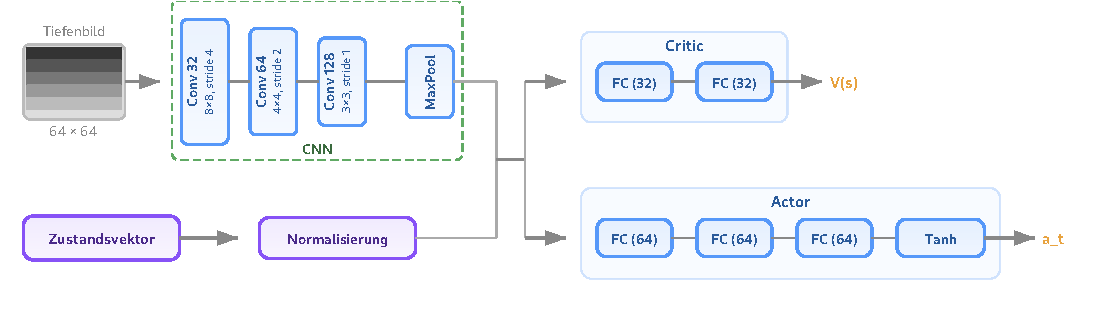
\includegraphics[width=\linewidth]{Bilder/architecture.pdf}
    \caption{Netzwerkarchitektur: Das Tiefenbild durchläuft einen geteilten
    CNN-Encoder (drei Faltungsschichten mit Batch-Normalisierung, ELU und
    abschließendem Global Max Pooling). Der resultierende 128-dimensionale
    Merkmalsvektor wird mit dem empirisch normalisierten Zustandsvektor
    konkateniert und an die getrennten MLP-Köpfe von Actor und Critic
    weitergegeben.}
    \label{fig:meth_architecture}
\end{figure}

\section{Trainingsverfahren}
\label{sec:meth_trainingsverfahren}

\subsection{Proximal Policy Optimization}
\label{subsec:meth_ppo}

Als Trainingsalgorithmus wird \emph{Proximal Policy Optimization} (PPO)
\autocite{schulmanProximalPolicyOptimization2017} eingesetzt, dessen Clipped Surrogate
Objective und vollständige Zielfunktion in Abschnitt~\ref{subsec:ppo_clip} eingeführt
wurden.

Die vorliegende Arbeit zielt auf einen kontinuierlichen Aktionsraum ab, in dem der Agent
Zielpositionsoffsets und eine Gierrate ausgibt (vgl.\
Abschnitt~\ref{subsec:meth_aktionsraum}). Wie in Abschnitt~\ref{subsec:ppo_clip} dargelegt,
übertrifft PPO auf strukturell vergleichbaren kontinuierlichen Steuerungsaufgaben die
Vergleichsverfahren TRPO und A2C. Auch im spezifischen
Anwendungsfeld der Drohnensteuerung hat sich PPO als Standardverfahren etabliert: Sowohl
\textcite{bartolomeiAutonomousEmergencyLanding2022} und
\textcite{xuNavRLLearningSafe2024} als auch
\textcite{kaufmannChampionlevelDroneRacing2023} setzen PPO ein
(vgl.\ Abschnitt~\ref{sec:architektur}). 
PPO passt zudem architektonisch zum gewählten
Trainingssetup: Als On-Policy-Verfahren verarbeitet es die gesammelten Daten direkt und
verwirft sie nach dem Update. Off-Policy-Verfahren wie SAC
\autocite{haarnojaOffPolicyMaximumEntropy2017} wurden daher verworfen. Sie erfordern
einen Replay Buffer, der vergangene Transitionen speichert und bei jedem Update erneut
abtastet. Ihre höhere Sample-Effizienz setzt zudem voraus, dass die Datensammlung der
Engpass ist. Bei GPU-paralleler Simulation mit hunderten bis tausenden Umgebungen ist
jedoch der Gradientenupdate der Engpass; die geringere Sample-Effizienz von
On-Policy-Methoden wird durch den Datendurchsatz mehr als kompensiert
\autocite{rudinLearningWalkMinutes2022}. Zudem würde ein Replay Buffer Transitionen aus
früheren Curriculum-Stufen enthalten (vgl.\
Abschnitt~\ref{subsec:meth_curriculum}), die für die aktuelle Stufe nicht mehr
repräsentativ sind.
Neuere PPO-Varianten wie Phasic Policy Gradient
\autocite{cobbePhrasicPolicyGradient2021} wurden nicht evaluiert, da die verwendete
Trainingsumgebung rsl-rl \autocite{rudinLearningWalkMinutes2022} ausschließlich die
Standard-PPO-Implementierung bereitstellt.

\subsubsection{Aktionsverteilung und Tanh-Squashing}
\label{subsubsec:meth_tanh_squashing}

Der Actor parametrisiert eine Gaußverteilung über einem unbeschränkten
Hilfsraum: Für jede Aktionsdimension~$i$ wird ein Rohwert
$u_i \sim \mathcal{N}(\mu_i, \sigma_i^2)$ gesampelt, wobei~$\mu_i$ und
$\log\sigma_i$ Netzausgaben sind. Der Aktionsraum ist jedoch auf $[-1,1]^4$
beschränkt (vgl.\ Abschnitt~\ref{subsec:meth_aktionsraum}). Ein naives
Clipping $a_i = \mathrm{clip}(u_i, -1, 1)$ würde die Aktionswerte korrekt
begrenzen, die zugehörige Log-Wahrscheinlichkeit jedoch weiterhin auf dem
unbeschnittenen Wert~$u_i$ berechnen. Da PPO das Verhältnis
$r_t(\theta) = \pi_\theta(\mathbf{a}_t \mid s_t) \,/\,
\pi_{\theta_{\mathrm{alt}}}(\mathbf{a}_t \mid s_t)$ zur Gradientenschätzung
nutzt (vgl.\ Abschnitt~\ref{subsec:ppo_clip}), führt diese Diskrepanz
zwischen ausgeführter und bewerteter Aktion zu verzerrten Gradienten.

Statt Clipping wird daher eine invertierbare, differenzierbare Transformation
verwendet~\autocite{haarnojaOffPolicyMaximumEntropy2017}:
\begin{equation} \label{eq:meth_tanh_squashing}
  a_i = \tanh(u_i).
\end{equation}
Die zugehörige Log-Wahrscheinlichkeit ergibt sich über die
Substitutionsregel für Wahrscheinlichkeitsdichten (Change of Variables):
\begin{equation} \label{eq:meth_tanh_logprob}
  \log\pi(\mathbf{a} \mid s)
  = \log\mathcal{N}(\mathbf{u} \mid \boldsymbol{\mu}, \boldsymbol{\sigma}^2)
  - \sum_{i=1}^{4} \log\!\bigl(1 - \tanh^2(u_i)\bigr).
\end{equation}
Der Korrekturterm~$-\sum_i \log(1 - \tanh^2(u_i))$ ist die
Log-Jacobi-Determinante der Tanh-Transformation und stellt sicher, dass die
Dichte im transformierten Raum korrekt normiert bleibt.

Zusätzlich erzwingt ein Floor $\log\sigma_i \geq -2{,}0$
($\sigma_i \geq 0{,}135$) eine Mindestexploration. Ohne diesen Floor kann PPO
die Standardabweichung gegen null treiben, was in der Log-Wahrscheinlichkeit zu
numerischen Instabilitäten führt und die Strategie irreversibel kollabieren
lässt.

\subsubsection{Hyperparameter}
\label{subsubsec:meth_hyperparams}

Tabelle~\ref{tab:meth_ppo_hyperparams} fasst die PPO-Hyperparameter zusammen.

\begin{table}[ht]
\centering
\caption{PPO-Hyperparameter der vorliegenden Arbeit.}
\label{tab:meth_ppo_hyperparams}
\small
\begin{tabular}{l l}
\toprule
\textbf{Parameter} & \textbf{Wert} \\
\midrule
Clipping $\varepsilon$      & $0{,}2$ \\
Diskontierung $\gamma$      & $0{,}99$ \\
GAE $\lambda$               & $0{,}95$ \\
Lernrate $\alpha$           & $5 \times 10^{-4}$ \\
Lern-Epochen $K$            & $5$ \\
Mini-Batches $M$            & $4$ \\
$c_1$ (Value-Loss)          & $1{,}0$ \\
$c_2$ (Entropie)            & $0{,}003$ \\
Gradient-Clipping           & $1{,}0$ \\
Schritte pro Env $T$        & $60$ \\
Parallele Envs $N$          & $256$ \\
Optimizer                   & Adam \\
\bottomrule
\end{tabular}
\end{table}

Die Werte für $\varepsilon$, $\gamma$, $\lambda$ sowie $K$ und
Gradient-Clipping entsprechen den von
\textcite{schulmanProximalPolicyOptimization2017} empfohlenen Standardwerten, die sich
in den MuJoCo-Benchmarks als robust über verschiedene Aufgaben erwiesen haben.
Der GAE-Parameter $\lambda = 0{,}95$ folgt der Empfehlung von
\textcite{schulmanHighDimensionalContinuousControl2016} als Kompromiss zwischen Bias und
Varianz. Die Lernrate $\alpha = 5 \times 10^{-4}$ wurde experimentell bestimmt:
Kleinere Werte führten zu sehr langsamer Konvergenz, größere zu kollabierenden
Strategien. Aufgabenspezifisch angepasst wurden ferner die Rollout-Länge~$T$ — 60~Entscheidungen
bei 3\,s Entscheidungsintervall ergeben 180\,s Rollout-Dauer — sowie die Anzahl
paralleler Umgebungen $N = 256$, begrenzt durch den GPU-Speicher der verwendeten
NVIDIA~A30 (24\,GB). Der Entropie-Koeffizient~$c_2 = 0{,}003$ wurde bewusst niedrig
gewählt, da die Tanh-Verteilung
(vgl.\ Abschnitt~\ref{subsubsec:meth_tanh_squashing}) empfindlich auf hohe Entropie-Anreize reagiert;
$c_2 \geq 0{,}01$ führte in Pilotexperimenten zu instabilem Training.

\section{Trainingsumgebung}
\label{sec:meth_trainingsumgebung}

\subsection{Physiksimulator}
\label{subsec:meth_simulator}

Das Training eines RL-Agenten vorliegende Aufgabe erfordert einen
Physiksimulator, der drei zentrale Anforderungen erfüllt:
(1)~GPU-parallelisierte Ausführung hunderter Umgebungsinstanzen, um die von PPO
benötigten großen Rollout-Batches effizient zu erzeugen
(vgl.\ Abschnitt~\ref{sec:meth_trainingsverfahren});
(2)~simulierte Tiefenkameras, da der Agent Tiefenbilder als Beobachtung erhält;
(3)~Import beliebiger 3D-Objekte, um realitätsnahe Hindernisszenarien zu
konstruieren.

Die vorliegende Arbeit verwendet Genesis
\autocite{xianGenesisUniversalGenerative2024}, einen 2024 veröffentlichten,
quelloffenen Physiksimulator für Robotik. Genesis erfüllt alle drei definierten
Anforderungen: Der Simulator führt bis zu 4096~Umgebungen GPU-parallel aus,
stellt Tiefenkameras über eine Batch-Rendering-Pipeline bereit, importiert
beliebige 3D-Meshes (u.\,a.\ URDF, OBJ) und bietet eine durchgängige
Python-API. Genesis zeichnet sich durch eine geringere Einstiegskomplexität aus:
Die Installation beschränkt sich auf ein einzelnes Python-Paket, und die API
erfordert keine herstellerspezifische Toolchain.

Gegenüber verbreiteten Alternativen bietet Genesis entscheidende Vorteile:
Gazebo \autocite{koenigDesignUseParadigms2004} und PyBullet
\autocite{coumansPybulletPythonModule2016} unterstützen keine GPU-parallele
Ausführung hunderter Umgebungen und scheiden daher für datenintensives
RL-Training aus. Isaac Gym \autocite{makoviychukIsaacGymHigh2021} erfüllt zwar
alle genannten Anforderungen, ist jedoch proprietär an NVIDIA gebunden und
erfordert einen umfangreichen Installationsstack.

Einschränkend ist anzumerken, dass Genesis mit seiner Erstveröffentlichung im
Dezember~2024 ein vergleichsweise junges Projekt ist und über eine kleinere
Community als etablierte Alternativen verfügt.

\subsection{Drohnenmodell}
\label{subsec:meth_drohne}

Die Drohne wird als URDF-Modell mit vier Rotoren simuliert. Die wesentlichen
physikalischen Parameter sind eine Masse von $0{,}714$\,kg, ein
Schub-Gewicht-Verhältnis von $2{,}25$ sowie eine Hover-Drehzahl von
$1789$\,RPM bei einer maximalen Drehzahl von $2700$\,RPM.

\subsection{Korridorgeometrie}
\label{subsec:meth_korridor}

Die Trainingsumgebung bildet einen vertikalen Korridor der Ausdehnung
$5 \times 2 \times 15$\,m ($x \times y \times z$) ab
(Abbildung~\ref{fig:meth_corridor}). Der Korridor besitzt keine physischen
Wände; stattdessen wird das Verlassen des Begrenzungsrahmens als Absturz
gewertet (vgl.\ Abschnitt~\ref{subsec:meth_terminierung}). Die Bodenebene
befindet sich bei $z = 0$\,m.

Die Drohne wird zu Episodenbeginn auf einer zufälligen Position im oberen
Korridorbereich bei $z = 12$\,m initialisiert, wobei die horizontale Position
gleichverteilt innerhalb von $\pm 1{,}5$\,m ($x$) bzw.\ $\pm 0{,}5$\,m ($y$)
um die Korridormitte variiert. Die Initialorientierung ist die Nulllage
(Quaternion $(1,0,0,0)$). Das Landeziel ist fixiert bei
$\mathbf{p}_{\mathrm{ziel}} = (0,\; 0,\; 1)^{\!\top}$\,m.

Während des Abstiegs durchquert die Drohne zwei horizontale Hindernisschichten
bei $z \approx 2$\,m und $z \approx 7$\,m
(vgl.\ Abschnitt~\ref{subsec:meth_hindernisse}).

\begin{figure}[ht]
    \centering
    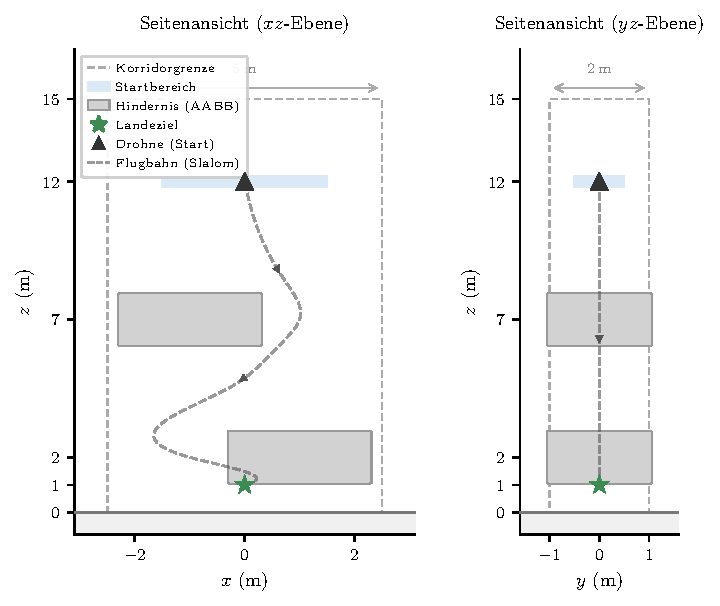
\includegraphics[width=0.85\linewidth]{Bilder/corridor_geometry.pdf}
    \caption{Seitenansichten der Korridorgeometrie. Links: $xz$-Ebene
    (Slalom-Achse) mit schematischer Flugbahn. Rechts: $yz$-Ebene. Die
    gestrichelten Rechtecke markieren die Korridorgrenzen, graue Flächen die
    schematischen Hindernis-Begrenzungsboxen.}
    \label{fig:meth_corridor}
\end{figure}

\subsection{Hindernisse}
\label{subsec:meth_hindernisse}

Als Hindernisse dienen sechs 3D-Objekte aus dem Google Scanned Objects
Datensatz~(GSO): eine Tasse, ein Teddybär, ein Spielzeugdinosaurier, ein
Spielzeugbus, ein Spielzeugnashorn und ein Schuh. Jedes Objekt wird um den
Faktor~$21$ bis~$63$ skaliert, sodass seine horizontale Ausdehnung mindestens
$2$\,m beträgt und damit die gesamte $y$-Breite des Korridors abdeckt. Objekte,
deren Höhe nach der Skalierung $2{,}0$\,m überschreitet, werden von unten
beschnitten.

Für die Kollisionserkennung und die Hindernisproximität
(vgl.\ Abschnitt~\ref{subsec:meth_belohnung}) wird die achsenparallele
Begrenzungsbox (AABB) jedes Objekts herangezogen. Diese konservative
Approximation umschließt das gesamte Mesh vollständig, sodass die Drohne
bereits vor Berührung der tatsächlichen Oberfläche als kollidiert gilt.

Die Platzierung folgt einem erzwungenen Slalom entlang der $x$-Achse: In jeder
der zwei Hindernisschichten wird ein zufällig gewähltes Objekt auf einer Seite
der Korridormitte positioniert, mit einem Versatz von $0{,}6$ bis $1{,}2$\,m.
Aufeinanderfolgende Schichten wechseln die Seite, sodass die Drohne einen
Slalomkurs fliegen muss. Die Startseite ($+x$ oder $-x$) wird pro Episode
zufällig gewählt.

\subsection{Verarbeitungspipeline}
\label{subsec:meth_pipeline}

Abbildung~\ref{fig:meth_pipeline} zeigt den vollständigen Datenfluss von der
Sensorik bis zur physikalischen Ausführung. Das normalisierte
Tiefenbild~$\mathbf{D}_t$ und der skalierte
Zustandsvektor~$\mathbf{o}_t$
(vgl.\ Abschnitt~\ref{subsec:meth_zustandsraum}) werden als
\texttt{TensorDict} gebündelt und der Actor-Critic-Architektur übergeben
(vgl.\ Abschnitt~\ref{sec:meth_architektur}). Die vom Actor gesampelte Aktion
wird gemäß Abschnitt~\ref{subsec:meth_aktionsraum} in Sollposition und
Sollgierwinkel skaliert und vom kaskadierenden PID-Regler
(vgl.\ Abschnitt~\ref{subsec:meth_uebergangsmodell}) über das
Entscheidungsintervall in Motordrehzahlen umgesetzt.

Sowohl das Tiefenbild als auch der Zustandsvektor werden direkt und
unverrauscht aus der Simulation erhoben. In einer realen Anwendung wären die
Tiefenbilder durch Sensorrauschen, Reflexionen und Ausfälle beeinflusst, und
die Zustandsinformationen müssten aus verrauschten IMU- und GPS-Messungen
geschätzt werden. Diese Idealisierung begrenzt die unmittelbare
Übertragbarkeit der trainierten Strategie auf reale Hardware.

\begin{figure}[ht]
    \centering
    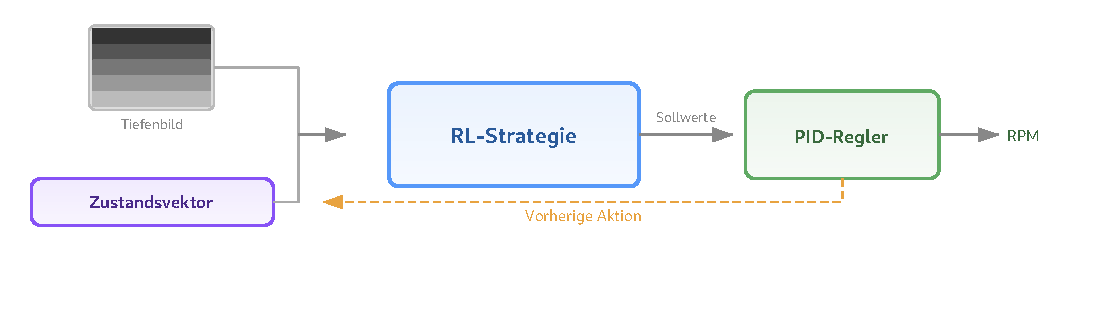
\includegraphics[width=\linewidth]{Bilder/pipeline.pdf}
    \caption{Verarbeitungspipeline: Tiefenbild und Zustandsvektor werden dem
    Actor-Netz (CNN~+~MLP) übergeben, das eine Aktion sampelt. Nach
    Skalierung steuert ein kaskadierender PID-Regler die Drohne über
    300~Simulationsschritte.}
    \label{fig:meth_pipeline}
\end{figure}

\subsection{Terminierung}
\label{subsec:meth_terminierung}

Eine Episode endet, wenn eine der folgenden Bedingungen eintritt:

\noindent\textbf{Erfolg.}\enspace Die Drohne verbleibt über die gesamte Dauer
eines Entscheidungsschritts ($3{,}0$\,s) innerhalb eines Radius von $0{,}5$\,m
um das Landeziel.

\noindent\textbf{Absturz.}\enspace Mindestens eine der folgenden Bedingungen
ist erfüllt:
\begin{itemize}
  \item Flughöhe $z < 0{,}2$\,m (Bodenkollision),
  \item Neigung $> 60^{\circ}$ in Roll oder Pitch (Kontrollverlust),
  \item AABB-Abstand zum nächsten Hindernis $< 0{,}3$\,m (Hinderniskollision),
  \item Verlassen des Korridors (Bounding-Box-Prüfung auf allen Achsen).
\end{itemize}

\noindent\textbf{Timeout.}\enspace Die maximale Episodenlänge von
$T_{\max} = 20$ Entscheidungsschritten ($60$\,s) ist erreicht. Timeouts werden
im Vorteilsschätzer als nicht-terminale Übergänge behandelt, sodass die
Wertfunktion den erwarteten Ertrag über die Episode hinaus approximiert.

\subsection{Curriculum}
\label{subsec:meth_curriculum}

Das Training folgt einem zweistufigen Curriculum. In der ersten Phase
(Iterationen~$0$ bis~$300$, entsprechend 18\,060~Entscheidungsschritten) sind
die Hindernisse deaktiviert, sodass der Agent zunächst den reinen Abstieg zum
Ziel erlernt. Die Korridorgrenzen sind von Beginn an aktiv. In der zweiten
Phase werden die Hindernisse bei jedem Episodenreset zufällig platziert und der
Agent muss sowohl die Navigation zum Ziel als auch die Hindernisvermeidung
bewältigen.
\chapter{Ergebnisse}
\label{cha:Ergebnisse}

\section{Trainingsverhalten}
\label{sec:trainingsverhalten}

Das Training wurde mit 512 parallelen Umgebungen auf einer NVIDIA A30 GPU
durchgeführt (341\,FPS Durchsatz) und nach 957~Iterationen durch die
24-Stunden-GPU-Zeitbegrenzung beendet.
Abbildung~\ref{fig:reward_training} zeigt den Belohnungsverlauf.

\begin{figure}[H]
    \centering
    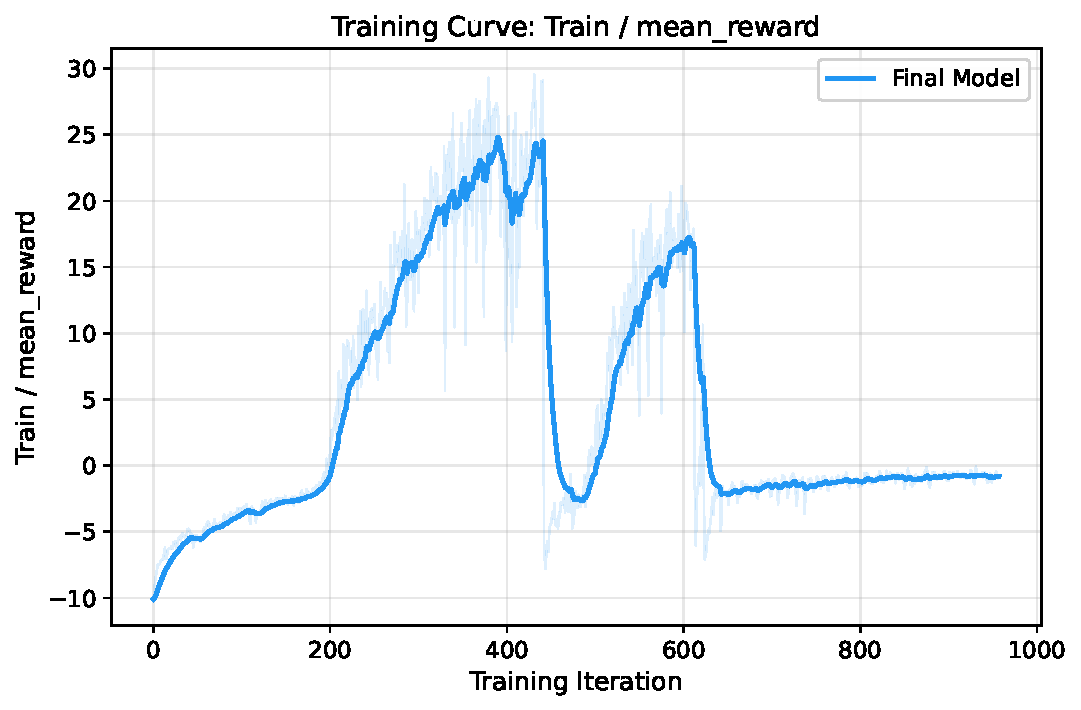
\includegraphics[width=0.48\textwidth]{figures/training/Train_mean_reward.pdf}
    \hfill
    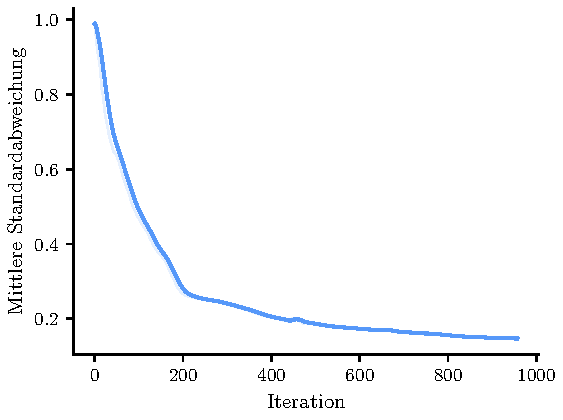
\includegraphics[width=0.48\textwidth]{figures/training/Policy_mean_std.pdf}
    \caption[Kumulative Belohnung und Standardabweichung der
    Aktionsverteilung]{Kumulative Belohnung (links) und mittlere
    Standardabweichung der Aktionsverteilung (rechts) über 957
    Trainingsiterationen. Geglättet mit EMA $\alpha = 0{,}9$,
    transparenter Hintergrund: Rohwerte.}
    \label{fig:reward_training}
\end{figure}

Der Trainingsverlauf lässt sich in zwei Phasen unterteilen. In der ersten
Phase (Iteration~0 bis~441) steigt die kumulative Belohnung kontinuierlich
an. Der Agent lernt zunächst die Zielnavigation; ab circa Iteration~200
erscheint erstmals die Erfolgsbelohnung
(Abbildung~\ref{fig:rew_crash_success}), und gleichzeitig sinkt die
Absturzrate. Die kumulative Belohnung erreicht ihren Höchstwert von 24,8
bei Iteration~390. Die Standardabweichung der Aktionsverteilung fällt
monoton von 0,99 auf 0,15, was die Konvergenz zu einer deterministischen
Strategie zeigt. Die übrigen Belohnungskomponenten bestätigen den
Lernfortschritt
(Abbildungen~\ref{fig:rew_eplen_close} und~\ref{fig:rew_prox_std} im
Anhang).

\begin{figure}[H]
    \centering
    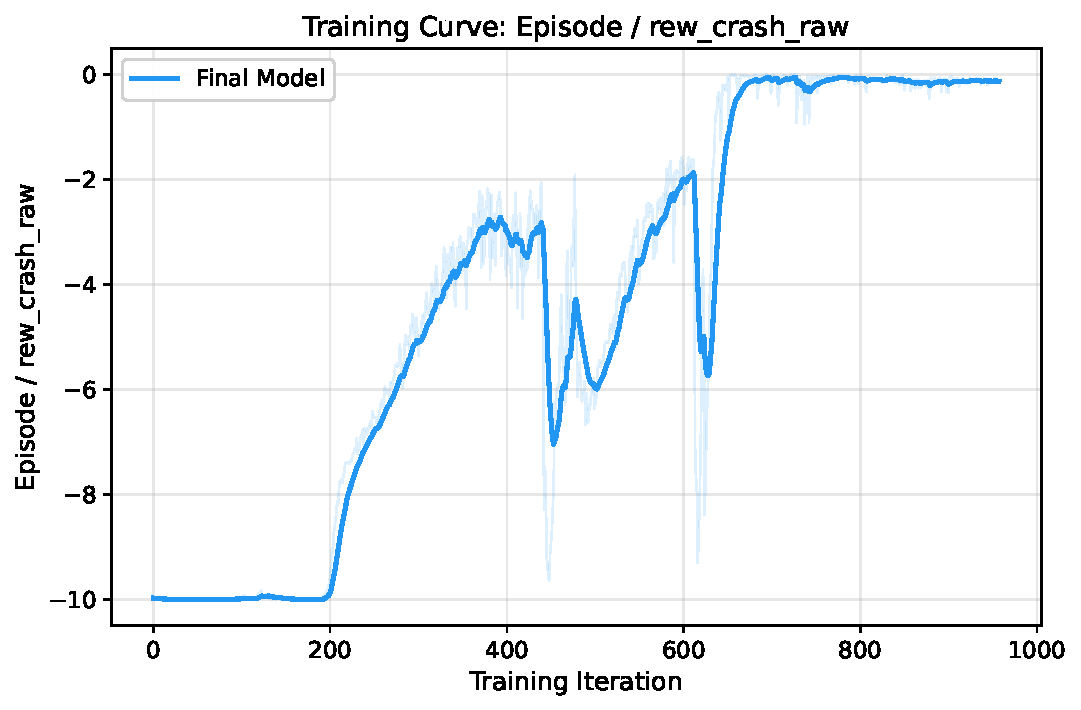
\includegraphics[width=0.48\textwidth]{figures/training/Episode_rew_crash_raw.pdf}
    \hfill
    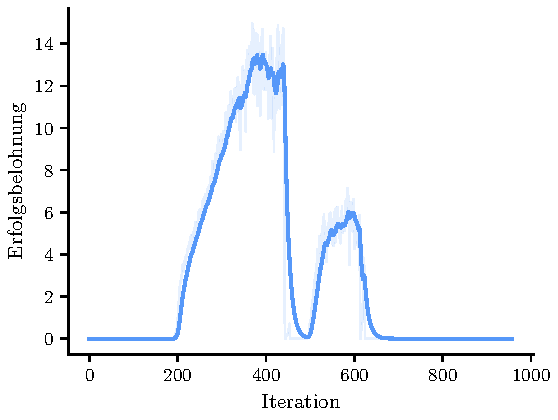
\includegraphics[width=0.48\textwidth]{figures/training/Episode_rew_success_raw.pdf}
    \caption[Absturzstrafe und Erfolgsbelohnung]{Unskalierte Absturzstrafe
    (links) und Erfolgsbelohnung (rechts). Geglättet mit EMA
    $\alpha = 0{,}9$.}
    \label{fig:rew_crash_success}
\end{figure}

Ab Iteration~442 bricht die kumulative Belohnung abrupt ein: Innerhalb einer
einzigen Iteration fällt sie von 29,2 auf $-6{,}1$. Die
Standardabweichung bleibt nahezu unverändert ($0{,}193 \rightarrow
0{,}194$); der Kollaps betrifft die Mittelwerte der Strategie, nicht die
Explorationsbreite.

Der beste Checkpoint liegt bei Iteration~400 (Tabelle~\ref{tab:konvergenz}).
Auf Basis des Belohnungsverlaufs wurde dieser für alle Evaluierungen
ausgewählt (\emph{Early Stopping}).

\begin{table}[H]
  \centering
  \caption[Konvergenzgeschwindigkeit und Checkpoint-Selektion]{Konvergenzgeschwindigkeit und Checkpoint-Selektion (512 Umgebungen, NVIDIA A30, 341\,FPS).}
  \label{tab:konvergenz}
  \small
  \renewcommand{\arraystretch}{1.1}
  \begin{tabular}{l r r r}
    \toprule
    \textbf{Checkpoint} & \textbf{Iteration} & \textbf{Laufzeit} & \textbf{Kum.\ Belohnung} \\
    \midrule
    Bestes Modell   & 400 & 10,4\,h & 23,0 \\
    Post-Kollaps    & 900 & 22,6\,h & $-1{,}1$ \\
    Trainingsende   & 957 & 24,0\,h & $-0{,}8$ \\
    \bottomrule
  \end{tabular}
\end{table}


\section{Phase 1: Korridornavigation}
\label{sec:phase1}

Versuchsreihe~1 (vgl.\ Abschnitt~\ref{subsec:meth_versuch1}) evaluiert die
trainierte Strategie (Checkpoint~400) über 1\,000~Episoden mit zuvor
ungesehenen Hindernisobjekten. Der Agent erreicht eine Erfolgsrate von
71,0\,\% (Abbildung~\ref{fig:phase1_outcomes}). Die fehlgeschlagenen
Episoden verteilen sich nahezu vollständig auf Hinderniskollisionen
(28,8\,\%); die verbleibenden 0,2\,\% enden durch Verlassen des
Korridors. Bodenkollisionen und Timeouts treten nicht auf.
Tabelle~\ref{tab:phase1_results} im Anhang listet alle Metriken mit
Konfidenzintervallen.

\begin{figure}[H]
    \centering
    
\includegraphics[width=0.65\textwidth]{figures/eval/phase1_outcomes.pdf}
    \caption[Episodenergebnisse Phase~1]{Episodenergebnisse der
    Phase-1-Evaluation (1\,000~Episoden). Fehlerbalken zeigen
    95\,\%-Bootstrap-Konfidenzintervalle.}
    \label{fig:phase1_outcomes}
\end{figure}

Das Flugverhalten zeigt zwei wiederkehrende Muster
(Abbildung~\ref{fig:phase1_trajectories}): Bei freier Bahn vollzieht der
Agent einen annähernd vertikalen Abstieg (mediane Pfadeffizienz 1,19). In
der Nähe eines Hindernisses bremst er spät ab und weicht lateral mit
geringem Sicherheitsabstand aus (mittlerer Minimalabstand 0,52\,m).

\begin{figure}[H]
    \centering
    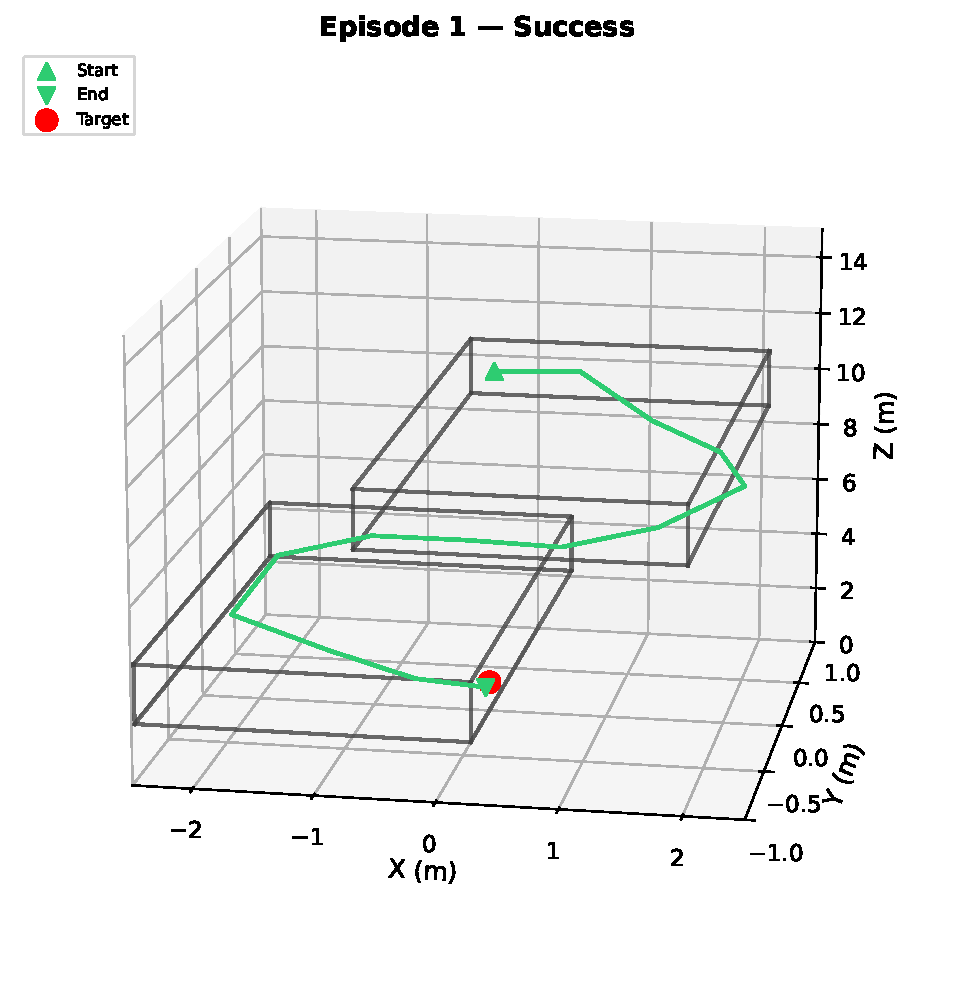
\includegraphics[width=0.32\textwidth]{figures/eval/trajectory_ep1.pdf}%
    \hfill
    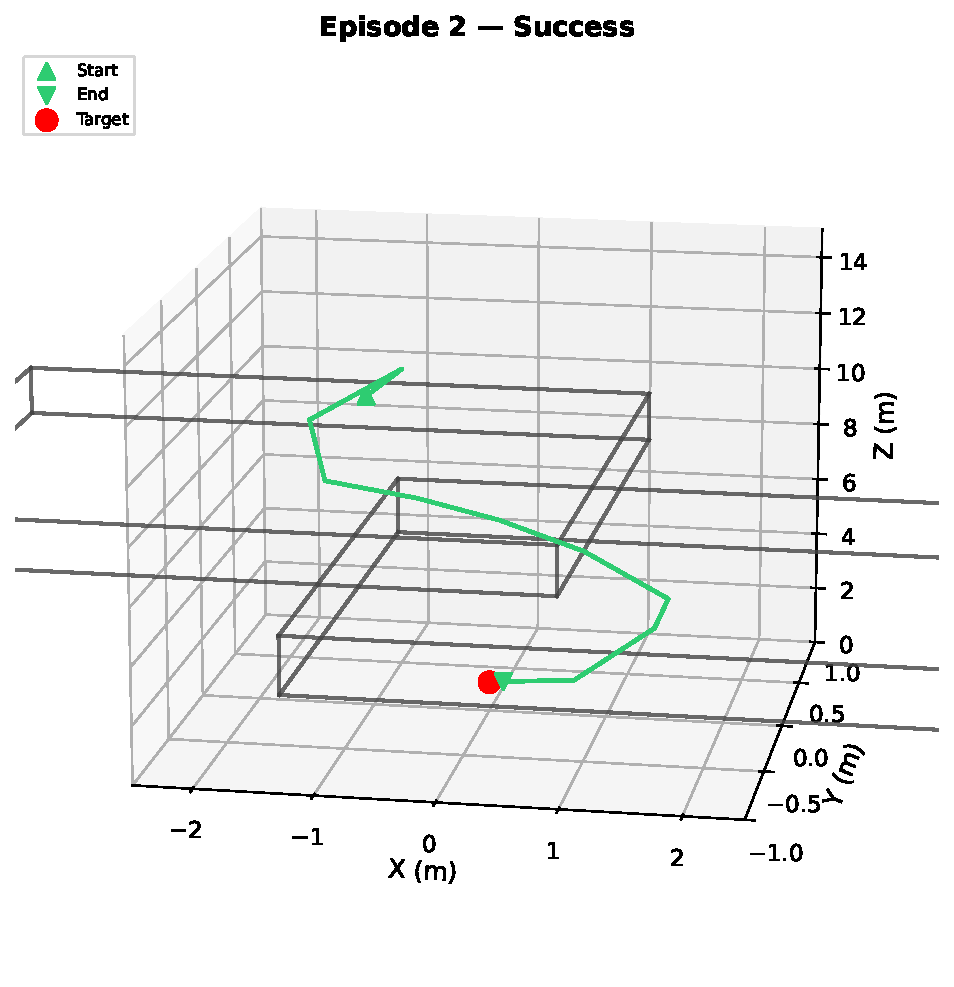
\includegraphics[width=0.32\textwidth]{figures/eval/trajectory_ep2.pdf}%
    \hfill
    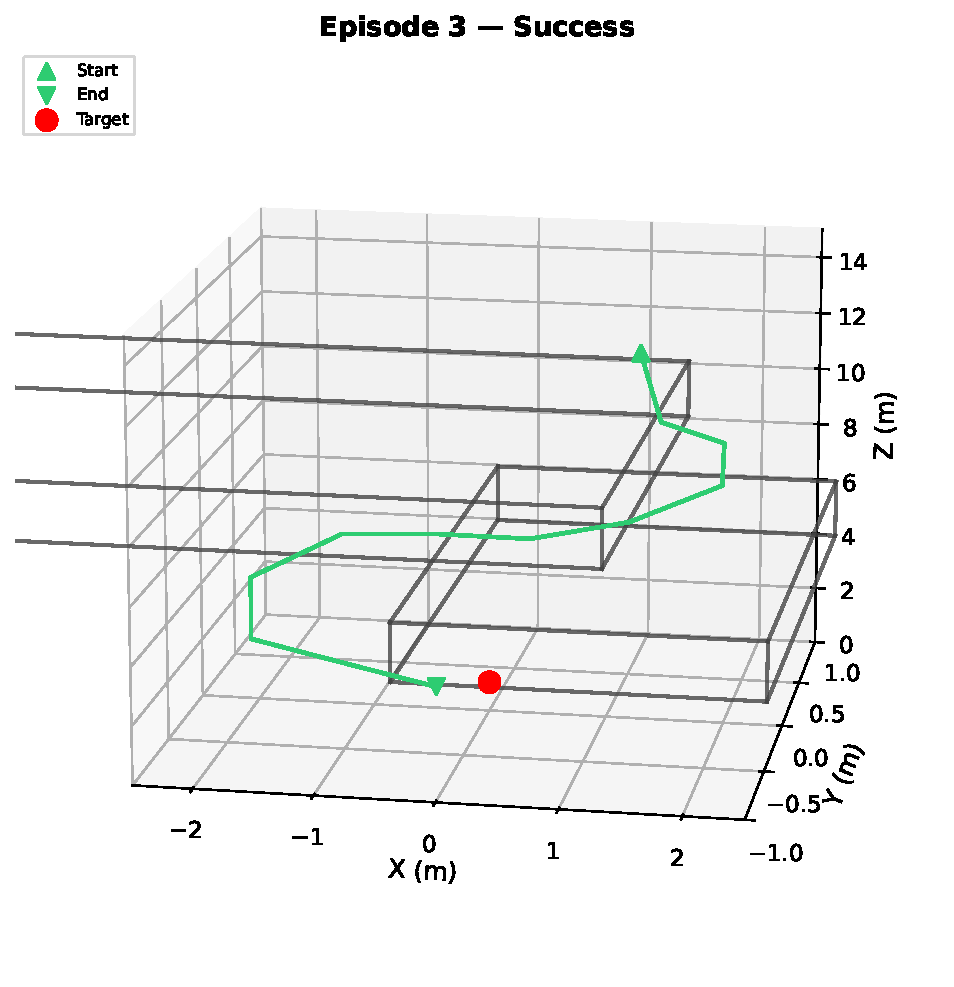
\includegraphics[width=0.32\textwidth]{figures/eval/trajectory_ep3.pdf}
    \caption[Exemplarische 3D-Trajektorien in Phase~1]{Exemplarische
    3D-Trajektorien dreier erfolgreicher Episoden. Graue Quader: AABB der
    Hindernisse. Grünes Dreieck: Startposition, roter Punkt: Landeziel.}
    \label{fig:phase1_trajectories}
\end{figure}

\subsection{Nachuntersuchung: Oberflächenbasierte Kollisionserkennung}
\label{subsec:phase1_mesh_contacts}

Das knappe Passieren bei hoher Kollisionsrate legte nahe, dass die
konservative AABB-Erkennung einen Teil der Fehlschläge verursacht. In
einer Nachuntersuchung mit 1\,000~Episoden wurde die
AABB-Kollisionserkennung durch die geometrisch exakte
Oberflächenkollisionsprüfung des Simulators ersetzt.

Mit oberflächenbasierter Kontakterkennung steigt die Erfolgsrate auf
98,4\,\% (Tabelle~\ref{tab:phase1_mesh_contacts}). Ein erheblicher
Anteil der AABB-Kollisionen sind demnach Fehlalarme: Die Drohne
durchfliegt die Begrenzungsbox, ohne die Oberfläche zu berühren.
Tabelle~\ref{tab:phase1_mesh_results} im Anhang listet alle Metriken.

\begin{table}[H]
  \centering
  \caption[Vergleich AABB- und oberflächenbasierte Kollisionserkennung]{Vergleich
  AABB-Distanz und oberflächenbasierte Kontakterkennung ($n = 1\,000$).}
  \label{tab:phase1_mesh_contacts}
  \small
  \renewcommand{\arraystretch}{1.1}
  \begin{tabular}{l r r}
    \toprule
    \textbf{Metrik} & \textbf{AABB} & \textbf{Oberfläche} \\
    \midrule
    Erfolgsrate                       & 71,0\,\%    & 98,4\,\% \\
    Hinderniskollision                & 28,8\,\%    & 1,2\,\% \\
    Verlassen des Korridors           & 0,2\,\%     & 0,2\,\% \\
    Timeout                           & 0,0\,\%     & 0,2\,\% \\
    \bottomrule
  \end{tabular}
\end{table}


\section{Phase 2: Weinberg-Transfer}
\label{sec:phase2}

Versuchsreihe~2 (vgl.\ Abschnitt~\ref{subsec:meth_versuch2}) evaluiert den
Zero-Shot-Transfer in die Weinbergumgebung über 1\,000~Episoden. Der Agent
erreicht eine Erfolgsrate von 10,4\,\%
(Abbildung~\ref{fig:phase2_outcomes}). Timeouts dominieren mit 73,7\,\%;
Terrain-Kollisionen verursachen 15,9\,\%. Der mediane Abstand zum
Landeziel am Episodenende beträgt 1,19\,m; 59,7\,\% der
Timeout-Episoden befinden sich innerhalb von 1,5\,m zum Ziel.
Tabelle~\ref{tab:phase2_results} im Anhang listet alle Metriken.

\begin{figure}[H]
    \centering
    
\includegraphics[width=0.65\textwidth]{figures/eval/phase2_outcomes.pdf}
    \caption[Episodenergebnisse Phase~2]{Episodenergebnisse der
    Phase-2-Evaluation (1\,000~Episoden, Zero-Shot-Transfer).
    Fehlerbalken zeigen 95\,\%-Bootstrap-Konfidenzintervalle.}
    \label{fig:phase2_outcomes}
\end{figure}

In der Mehrzahl der Fälle erreicht der Agent die Umgebung des Landeziels,
verbleibt jedoch außerhalb des Erfolgsradius von 0,5\,m mit ineffektiven
Korrekturbewegungen.

\subsection{Sensitivitätsanalyse des Erfolgskriteriums}
\label{subsec:phase2_relaxed}

Mit einem erweiterten Erfolgsradius von 1,5\,m steigt die Erfolgsrate auf
69,7\,\% (Tabelle~\ref{tab:phase2_relaxed}). Die
Terrain-Kollisionsrate sinkt von 15,9\,\% auf 9,4\,\%, da ein Teil der
zuvor als Timeout gewerteten Episoden nun frühzeitig als Erfolg beendet
wird. Der Timeout-Anteil sinkt von 73,7\,\% auf 27,7\,\%.

\begin{table}[H]
  \centering
  \caption[Sensitivitätsanalyse des Erfolgsradius in Phase~2]{Sensitivitätsanalyse
  des Erfolgsradius~$r$ in der Weinbergumgebung ($n = 1\,000$ je Bedingung).}
  \label{tab:phase2_relaxed}
  \small
  \renewcommand{\arraystretch}{1.1}
  \begin{tabular}{l r r}
    \toprule
    \textbf{Metrik} & \textbf{$r = 0{,}5$\,m} & \textbf{$r = 1{,}5$\,m} \\
    \midrule
    Erfolgsrate           & 10,4\,\%    & 69,7\,\% \\
    Terrain-Kollision     & 15,9\,\%    & 9,4\,\% \\
    Timeout               & 73,7\,\%    & 27,7\,\% \\
    \bottomrule
  \end{tabular}
\end{table}


\section{Vergleich RL vs.\ RRT-Connect}
\label{sec:vergleich_rl_rrt}

Der RRT-Planer übertrifft den RL-Agenten in der Erfolgsrate beider
Umgebungen, wobei der Abstand im Weinberg deutlich größer ausfällt. Im
Korridor dominieren bei beiden Verfahren Hinderniskollisionen; im Weinberg
scheitert der RL-Agent überwiegend an Timeouts (73,7\,\%), während der
RRT-Planer diese auf 7,9\,\% begrenzt. Der RL-Agent landet schneller
(30,0\,s gegenüber 42,0\,s im Korridor).\footnote{Einzelne
Pfadeffizienzwerte knapp unter 1,0 sind ein Implementierungsartefakt:
Das letzte Flugsegment wird aufgrund des automatischen Zurücksetzens der
Umgebung nicht erfasst.} Dem steht ein einmaliger Trainingsaufwand von
circa 24~Stunden gegenüber. Detaillierte Metriken mit
Konfidenzintervallen finden sich in den
Anhangstabellen~\ref{tab:phase1_results} und~\ref{tab:phase2_results}. Tabelle~\ref{tab:vergleich_rl_rrt} stellt die Ergebnisse beider Verfahren
gegenüber.

\begin{table}[H]
  \centering
  \caption[Vergleich RL-Agent und RRT-Connect]{Vergleich von RL-Agent und
  RRT-Connect über beide Versuchsreihen ($n = 1\,000$ je Bedingung).}
  \label{tab:vergleich_rl_rrt}
  \footnotesize
  \renewcommand{\arraystretch}{1.15}
  \begin{tabular}{l r r r r}
    \toprule
    & \multicolumn{2}{c}{\textbf{Phase~1 (Korridor)}}
    & \multicolumn{2}{c}{\textbf{Phase~2 (Weinberg)}} \\
    \cmidrule(lr){2-3} \cmidrule(lr){4-5}
    \textbf{Metrik}
      & \textbf{RL} & \textbf{RRT}
      & \textbf{RL} & \textbf{RRT} \\
    \midrule
    Erfolgsrate
      & 71,0\,\%       & 82,0\,\%
      & 10,4\,\%       & 85,7\,\% \\
    \quad(relaxed $r = 1{,}5$\,m)
      & \multicolumn{2}{c}{n.\,a.}
      & 69,7\,\%       & 98,4\,\% \\
    \addlinespace
    Hindernis-/Terrain-Koll.
      & 28,8\,\%       & 18,0\,\%
      & 15,9\,\%       & 7,1\,\% \\
    Timeout
      & 0,0\,\%        & 0,0\,\%
      & 73,7\,\%       & 7,9\,\% \\
    \addlinespace
    Landezeit (Median)
      & 30,0\,s         & 42,0\,s
      & 36,0\,s         & 42,0\,s \\
    Pfadeffizienz (Median)
      & 1,19            & 1,09
      & 1,07            & 0,99 \\
    Min.\ Abstand (Mittel)
      & 0,52\,m         & 0,48\,m
      & 1,02\,m         & 0,46\,m \\
    \bottomrule
  \end{tabular}
\end{table}
\chapter{Diskussion}
\label{cha:Diskussion}

Dieses Kapitel interpretiert die in Kapitel~\ref{cha:Ergebnisse} berichteten
Ergebnisse im Kontext der vier Nebenfragestellungen. Jeder Abschnitt schließt
mit einer expliziten Antwort auf die zugehörige Fragestellung.

\section{Leistungsfähigkeit in der Trainingsumgebung}
\label{sec:disk_nf1}

\subsection{Trainingsverhalten und Konvergenz}

Die zwei beobachteten Phasen im Belohnungsverlauf lassen sich auf die
Belohnungsstruktur zurückführen, die dichte Komponenten mit
ereignisbasierten Boni kombiniert. In der Konvergenzphase (Iteration~0
bis~441) ermöglichen die dichten Komponenten ($r_{\mathrm{prog}}$,
$r_{\mathrm{nah}}$, $r_{\mathrm{prox}}$) den initialen Anstieg, indem
sie bereits für Teilfortschritte Signal liefern. Ab circa Iteration~200
setzt zusätzlich die Erfolgsbelohnung $r_{\mathrm{erf}}$ ein, sobald der
Agent erstmals konsistente Landungen erreicht, und beschleunigt den
Belohnungsanstieg. Ohne die dichten Komponenten würde dem Agenten in der
frühen Trainingsphase das Gradientensignal für Teilfortschritte fehlen,
was die Konvergenz vermutlich erheblich verzögern würde. Der abrupte Kollaps ab Iteration~442 betrifft ausschließlich die
Mittelwerte der Strategie bei nahezu unveränderter Standardabweichung
($0{,}193 \rightarrow 0{,}194$), was auf eine katastrophale
Strategieaktualisierung hindeutet, nicht auf einen graduellen
Stabilitätsverlust. Obwohl der Clipping-Mechanismus von
PPO~\autocite{schulmanProximalPolicyOptimization2017} große
Strategieänderungen pro Iteration begrenzen soll, reicht er nicht aus,
um solche abrupten Einbrüche zu verhindern. Eine mögliche Erklärung
bieten \textcite{moallaNoRepresentationNoTrust2024}, die zeigen, dass
eine schleichende Verschlechterung des Feature-Ranks im
Actor-Netzwerk den Clipping-Mechanismus unterlaufen und zu
unumkehrbaren Leistungseinbrüchen führen kann, wobei die
Standardabweichung als globaler Parameter unbeeinflusst bleibt. Ob
dieser Mechanismus den beobachteten Kollaps erklärt, lässt sich ohne
Analyse des Feature-Ranks nicht abschließend beurteilen. % REVIEW: Moalla et al. 2024 (NeurIPS) — Quelle lesen und bestätigen

Die im Trainingsverlauf ansteigende Landezeit lässt sich auf die
Struktur der Belohnungsfunktion zurückführen. Die beiden dominanten
Komponenten Fortschritt $r_{\mathrm{prog}}$ (Gewicht~$1{,}0$) und Nähe
$r_{\mathrm{nah}}$ (Gewicht~$2{,}0$) werden bei steilem Sinkflug
maximiert, da die 3D-Distanz zum Ziel pro Schritt am stärksten abnimmt.
Entscheidend ist dabei die unterschiedliche Natur beider Komponenten:
$r_{\mathrm{prog}} = d_{t} - d_{t+1}$ misst die Distanzverringerung pro
Schritt und ist damit potentialbasiert im Sinne von
\textcite{ngPolicyInvarianceReward1999}; solches Reward Shaping
verändert die optimale Strategie nicht.
$r_{\mathrm{nah}} = \exp(-d_{t+1})$ hingegen ist nicht potentialbasiert,
sondern ein zustandsabhängiger Pro-Schritt-Reward: Jeder Zeitschritt in
Zielnähe liefert Belohnung, unabhängig davon, ob der Agent sich dem Ziel
weiter nähert. Da die Zeitstrafe deaktiviert ist (Gewicht~$0{,}0$),
existiert kein Gegengewicht zu diesem Verweil-Anreiz. Dieses Phänomen
ist in der Literatur bekannt: \textcite{randlovLearningDriveBicycle1998}
dokumentieren, dass ein nicht-potentialbasierter Shaping-Reward einen
Agenten dazu bringt, Kreise zu fahren statt das Ziel zu erreichen, da
die akkumulierte Zwischenbelohnung die Zielbelohnung übersteigt. % REVIEW: Randlov & Alstrom 1998 (ICML) — Quelle lesen und bestätigen
Der Agent lernt folglich eine Strategie, die steilen Abstieg mit
ausgedehntem Schweben in Zielnähe kombiniert, was die beobachtete
Zunahme der Episodenlänge im Trainingsverlauf erklärt.

\subsection{Dominante Fehlerart und Flugverhalten}

Die Failure-Mode-Analyse zeigt ein eindeutiges Bild:
Hinderniskollisionen verursachen 28,8\,\% aller Episodenausgänge und
stellen damit die einzig relevante Fehlerart dar. Zeitüberschreitungen und
Bodenkollisionen treten nicht auf (jeweils 0,0\,\%); der Agent erreicht
in jeder Episode die Zielumgebung. Die Nachuntersuchung mit
oberflächenbasierter Kollisionserkennung
(Abschnitt~\ref{subsec:phase1_mesh_contacts}) relativiert dieses
Ergebnis: Mit geometrisch exakter Kontaktprüfung steigt die Erfolgsrate
auf 98,0\,\%, was zeigt, dass der Großteil der registrierten Kollisionen
auf die konservative AABB-Metrik zurückgeht und nicht auf tatsächliche
Berührungen der Hindernisoberfläche. Der limitierende Faktor der
berichteten 71,0\,\% Erfolgsrate ist somit primär die Kollisionsmetrik,
nicht das erlernte Flugverhalten.

Zur Einordnung: \textcite{bartolomeiAutonomousEmergencyLanding2022}
berichten vergleichbare Erfolgsraten (über 70\,\%) für ein RL-System mit
Tiefenbildeingabe und diskretem Aktionsraum. Deren Aufgabe ist jedoch
die Selektion sicherer Landezonen in offenem Gelände, nicht die
Navigation durch Hindernisse zu einem festen Ziel. Dass der hier
trainierte Agent mit kontinuierlichem Aktionsraum in einer
Korridorumgebung mit erzwungenen Ausweichmanövern vergleichbare Raten
erreicht, spricht für die Leistungsfähigkeit der gewählten Architektur.

Das qualitative Flugverhalten ist reaktiv: Der Agent nähert sich einem
Hindernis auf direktem Weg, bremst auf kurzer Distanz ab, weicht lateral
aus und setzt den Abstieg fort. Dieses Muster ist eine direkte Konsequenz
des begrenzten lokalen Sensorhorizonts: Die nach unten gerichtete Kamera
erfasst Hindernisse erst bei relativer Nähe, sodass vorausschauende
Planung nicht möglich ist. \textcite{chenDRQN3DObstacleAvoidance2021}
zeigen, dass Agenten mit eingeschränktem Sichtfeld ohne temporales
Gedächtnis zwangsläufig reaktives Ausweichverhalten im letzten Moment
entwickeln; erst eine LSTM-Erweiterung ermöglicht vorausschauendes
Handeln. Die hier eingesetzte CNN-MLP-Architektur ohne rekurrente
Komponente ist daher strukturell auf reaktives Verhalten beschränkt. % REVIEW: Chen et al. 2021 (IROS) — Quelle lesen und bestätigen Bemerkenswert ist die
Präzision, mit der Hindernisse in geringem Abstand passiert werden
(mittlerer Minimalabstand 0,52\,m bei einem Kollisionsradius von
0,3\,m).

\subsection{Perceptual Aliasing}

Ein fundamentales Problem der gewählten Sensorarchitektur zeigt sich
unmittelbar in den aufgezeichneten Tiefenbildern: Boden und Hindernisse
erzeugen bei Annäherung nahezu identische Tiefensignaturen. Während die
Annäherung an den Boden das Ziel darstellt, muss jene an Hindernisse
vermieden werden. Der Agent löst diese Ambiguität implizit: Die relative
Positionsinformation im Zustandsvektor kodiert die Entfernung zum Ziel und
damit indirekt die erwartete Flughöhe, sodass das Modell lernen kann, ob
eine abnehmende Tiefe Boden oder Hindernis bedeutet.
\textcite{bartolomeiAutonomousEmergencyLanding2022} adressieren dieses
Problem, indem sie neben Tiefenbildern zusätzlich semantische
Segmentierungen als Eingabe verwenden, die eine explizite Unterscheidung
von Oberflächentypen ermöglichen. Im vorliegenden System steht eine
solche Segmentierung nicht zur Verfügung; die Disambiguierung stützt
sich ausschließlich auf den Zustandsvektor.

\subsection{Beantwortung NF1}

Der trainierte Agent erreicht in der Korridorumgebung eine Erfolgsrate
von 71,0\,\% unter der konservativen AABB-Kollisionsmetrik; mit
oberflächenbasierter Kontakterkennung steigt dieser Wert auf 98,0\,\%.
Hinderniskollisionen (28,8\,\%) sind die einzig relevante Fehlerart,
wobei der Großteil auf die Konservativität der AABB-Metrik
zurückzuführen ist. Der Agent erlernt eine reaktive Ausweichstrategie,
die Hindernisse mit hoher Präzision passiert. Ihre Leistungsgrenze wird
primär durch den begrenzten Sensorhorizont der nach unten gerichteten
Tiefenkamera bestimmt. Die nicht-potentialbasierte
Nähebelohnung $r_{\mathrm{nah}}$ erzeugt dabei einen Verweil-Anreiz in
Zielnähe, der die Landezeiten erhöht, aber die geforderte Landepräzision
begünstigt.

\section{Transferleistung auf den Weinberg}
\label{sec:disk_nf2}

\subsection{Success-Drop und Failure-Mode-Shift}

Der Leistungsabfall von Phase~1 zu Phase~2 ist erwartbar: Der Agent wurde
ausschließlich in der Korridorumgebung trainiert und sieht die
Weinberggeometrie erstmals zur Evaluationszeit. Aufschlussreich ist weniger
der Drop selbst als dessen Zusammensetzung.
% TODO: Interpretation je nach dominantem Failure-Mode einfügen.
% Falls Timeouts dominieren: Ein erhöhter Timeout-Anteil deutet darauf hin,
% dass der Agent sich dem Ziel zwar nähert, aber in der Nähe der Landefläche
% kein stabiles Hovern erreicht.
% Falls Terrain-Kollisionen dominieren: Die Verschiebung von
% Hinderniskollisionen zu Terrain-Kollisionen spiegelt den geometrischen
% Unterschied der Umgebungen wider.

\subsection{Einordnung als Sim-to-Sim Transfer}

Die Phase-2-Evaluation ist als Zero-Shot Sim-to-Sim Transfer einzuordnen:
Der Agent wird ohne Fine-Tuning und ohne Domain Randomization in einer
geometrisch verschiedenartigen Umgebung evaluiert. Dass überhaupt eine
partielle Übertragbarkeit besteht, lässt sich auf die umgebungsagnostische
Beobachtungsstruktur zurückführen. Der Zustandsvektor kodiert relative
Positionen, und das Tiefenbild enthält keine texturbasierten Merkmale, die
an die Korridorgeometrie gebunden wären. Diese Einordnung sollte nicht
überbewertet werden: Sim-to-Sim Transfer unter kontrollierten Bedingungen
ist ein schwächeres Ergebnis als Sim-to-Real Transfer oder Generalisierung
über diverse Trainingsumgebungen.

\subsection{Perceptual Aliasing im Weinberg}

Das in Abschnitt~\ref{sec:disk_nf1} beschriebene Perceptual-Aliasing-Problem
bietet eine Erklärung für die erhöhte Terrain-Kollisionsrate im Weinberg. Im
Korridor ist die Landefläche hindernisfrei: Sobald der Agent die letzte
Hindernisschicht passiert hat, kann er das Tiefenbild in der terminalen Phase
gefahrlos ignorieren und sich ausschließlich am Zustandsvektor orientieren.
Dass der Agent genau diese Strategie erlernt, ist plausibel, da das
Tiefenbild in Bodennähe ohnehin nur noch abnehmendes Bodenrelief zeigt und
keinen handlungsrelevanten Informationsgewinn bietet. Im Weinberg bricht
diese Strategie: Rebenreihen ragen als vertikale Strukturen direkt in die
Landezone, sodass die Tiefenwahrnehmung gerade in der terminalen Phase
entscheidungsrelevant bleibt. Ein Agent, der gelernt hat, das Tiefenbild in
Zielnähe zu ignorieren, kollidiert mit Vegetation, die er bei aktiver
Auswertung hätte umgehen können.

Ein möglicher Lösungsansatz wäre die Ergänzung der Beobachtung um eine
semantische Segmentierung, die Boden, Hindernisse und Vegetation als separate
Klassen ausweist. Anstatt die Boden-Hindernis-Unterscheidung implizit aus dem
Tiefenbild ableiten zu müssen, könnte der Agent direkt lernen, welche
Strukturen gefahrlos überflogen werden dürfen und welche ein Ausweichmanöver
erfordern.

\subsection{Beantwortung NF2}

% TODO: Explizite Antwort auf NF2 einfügen. Beispielstruktur:
% Die erlernte Navigationsleistung lässt sich partiell auf die
% Weinbergumgebung übertragen: Die Erfolgsrate sinkt von [X\,\%] auf
% [Y\,\%], wobei sich der dominante Failure-Mode von [A] zu [B]
% verschiebt. Der Transfer gelingt ohne Fine-Tuning, ist aber durch das
% verschärfte Perceptual-Aliasing-Problem in der terminalen Landephase
% begrenzt.

\section{Leistungslücke zum Pfadplaner}
\label{sec:disk_nf3}

\subsection{Inferenzzeit und Echtzeitfähigkeit}

Ein entscheidender praktischer Vorteil des RL-Agenten liegt in der
Inferenzzeit. Ein Forward-Pass durch das Netzwerk benötigt konstante Zeit
unabhängig von der Umgebungskomplexität, während RRT-Connect iterativ Pfade
sampelt und Kollisionsprüfungen auswertet. Auf eingebetteter Hardware, wie
sie für reale Drohnenanwendungen relevant wäre, ist der RL-Agent
echtzeitfähig, während RRT-Connect entweder ein stark begrenztes Sampling-Budget
oder leistungsfähigere Hardware erfordert.

\subsection{Landegeschwindigkeit}

Die in Abschnitt~\ref{subsec:meth_versuch1} beschriebene
Informationsasymmetrie lässt eine deutliche Leistungslücke zugunsten des
RRT-Connect-Planers erwarten. Dass der RL-Agent dennoch vergleichbare Erfolgsraten
erzielt, zeigt, dass die implizite Hindernisrepräsentation im Tiefenbild
für diese Aufgabe ausreichend ist. Der RL-Agent erzielt zudem kürzere
Landezeiten: Er lernt direkte Trajektorien, die keine konservativen
Sicherheitsabstände einhalten, wie sie ein sampling-basierter Planer
typischerweise produziert.

\subsection{Planungshorizont}

RRT-Connect plant global: Der gesamte Pfad wird vor Flugbeginn berechnet. Der
RL-Agent entscheidet lokal, pro Zeitschritt, auf Basis der aktuellen
Beobachtung. In dieser Arbeit sind alle Hindernisse statisch, sodass der
globale Planungshorizont von RRT-Connect ein reiner Vorteil ist. In dynamischen
Umgebungen kehrt sich dieses Verhältnis um: RRT-Connect müsste bei jeder Änderung
replanen, während der RL-Agent durch seine lokale Entscheidungsstruktur
inhärent auf veränderte Bedingungen reagieren kann. Dieses Argument bleibt
im Kontext dieser Arbeit theoretisch, ist aber für die praktische
Motivation des lernbasierten Ansatzes relevant.

\subsection{Beantwortung NF3}

% TODO: Explizite Antwort auf NF3 einfügen. Beispielstruktur:
% Die Leistungslücke zwischen RL-Agent und RRT-Connect-Pfadplaner beträgt
% [X Prozentpunkte] in der Erfolgsrate. Der RL-Agent kompensiert diese
% Differenz durch kürzere Landezeiten und Echtzeitfähigkeit.

\section{Beitrag der Beobachtungskomponenten}
\label{sec:disk_nf4}

Eine quantitative Beantwortung von NF4 erfordert eine Ablationsstudie,
in der ein State-only-Modell (ohne Tiefenbild) unter identischen
Bedingungen trainiert und evaluiert wird. Eine solche Ablation wurde im
Rahmen dieser Arbeit nicht durchgeführt; der individuelle Beitrag von
Tiefenwahrnehmung und propriozeptivem Zustandsvektor lässt sich daher
nur indirekt abschätzen.

Das beobachtete Flugverhalten liefert qualitative Hinweise: Die
lateralen Ausweichmanöver vor Hindernissen
(Abschnitt~\ref{sec:phase1}) setzen Hindernisinformation voraus, die
ausschließlich im Tiefenbild enthalten ist, da der Zustandsvektor keine
Hindernispositionen kodiert. Ohne visuelle Eingabe könnte der Agent
lediglich den direkten Abstieg zum Ziel erlernen; erfolgreiche Episoden
wären auf Hinderniskonfigurationen beschränkt, die zufällig einen freien
Korridor auf der Abstiegslinie belassen. Die Transferleistung auf
unbekannte Hindernisformen (Phase~1) und auf die Weinbergumgebung
(Phase~2) stützt die Hypothese, dass das CNN geometrische Strukturen
erkennt, die über die Trainingsumgebung hinaus generalisieren. Welche
konkreten Merkmale extrahiert werden, bleibt ohne
Feature-Visualisierung (z.\,B.\ Grad-CAM) offen.

\subsection{Beantwortung NF4}

Die Frage nach dem individuellen Beitrag der Beobachtungskomponenten
kann ohne Ablationsstudie nicht quantitativ beantwortet werden. Die
qualitative Analyse des Flugverhaltens legt nahe, dass die
Tiefenwahrnehmung die Hindernisumgehung ermöglicht, während der
Zustandsvektor die Zielnavigation und den kontrollierten Abstieg
steuert. Eine experimentelle Validierung dieser Hypothese bleibt
zukünftiger Arbeit vorbehalten
(vgl.\ Abschnitt~\ref{sec:disk_limitationen}).

\section{Limitationen}
\label{sec:disk_limitationen}

\textbf{Einzelner Seed.}
Alle Ergebnisse basieren auf einem einzigen Trainingslauf. Die
Bootstrap-Konfidenzintervalle quantifizieren die Evaluationsvarianz über
Hinderniskonfigurationen und Startpositionen, nicht die Trainingsvarianz.
Ein anderer Seed könnte zu qualitativ anderem Verhalten führen. Die
berichteten Erfolgsraten sind daher als Punktschätzung eines einzelnen
Trainingslaufs zu verstehen, nicht als robuste Aussage über die Methode.

\textbf{Sim-to-Real Gap.}
Die Simulation bietet perfekte Sensorik ohne Rauschen, keine
Windeinflüsse, keine Motorverzögerung und keine Kommunikationslatenz.
Ergebnisse sind nicht direkt auf reale Drohnen übertragbar. Es wurde kein
Domain-Randomization-Ansatz implementiert, der die Robustheit gegenüber
sensorischen Störungen erhöhen könnte.

\textbf{Reward Shaping.}
Die Belohnungsgewichte wurden manuell in Vorversuchen abgestimmt. Andere
Gewichtungen könnten zu qualitativ anderem Verhalten führen. Ein
systematisches Hyperparameter-Tuning der Reward-Gewichte wurde nicht
durchgeführt.

\textbf{Feste Zielposition.}
Das Landeziel ist in allen Episoden identisch. Obwohl die Beobachtung
relativ kodiert ist, könnte der Agent auf positionsspezifische Muster
überangepasst sein.

\textbf{Statische Umgebung.}
Alle Hindernisse sind statisch. Reale Weinberge weisen bewegliche
Vegetation, Wind und andere dynamische Elemente auf.

\textbf{Keine Ablation und keine Feature-Visualisierung.}
Der individuelle Beitrag von Tiefenwahrnehmung und Zustandsvektor wurde
nicht durch eine Ablationsstudie quantifiziert
(vgl.\ Abschnitt~\ref{sec:disk_nf4}). Die Schlussfolgerungen über die
gelernten CNN-Repräsentationen sind indirekt aus Trajektorien und
Transferleistung abgeleitet. Eine Grad-CAM-Analyse oder vergleichbare
Methode würde direktere Evidenz liefern.

\chapter{Fazit und Ausblick}
\label{cha:Fazit und Ausblick}

\section{Beantwortung der Forschungsfragen}

Die vorliegende Arbeit untersuchte, inwiefern ein RL-basierter Ansatz eine
autonome Drohne befähigen kann, mithilfe lokaler Tiefensensorik in
hindernisreichen Umgebungen sicher zu landen.

Der trainierte Agent erlernt eine reaktive Ausweichstrategie, deren
Leistung primär durch strukturelle Entwurfsentscheidungen begrenzt wird:
Sensorhorizont, Entscheidungsintervall und Belohnungsgewichtung bestimmen,
wie knapp der Agent Hindernisse passiert. Die Wahl der Kollisionsmetrik
erweist sich als entscheidender Faktor: Unter oberflächenbasierter
Erkennung erreicht der Agent 98,4\,\% und übertrifft damit den
privilegierten Pfadplaner (82,0\,\%).

Die Transferuntersuchung zeigt eine klare Trennung zweier
Teilfähigkeiten: Hindernisnavigation generalisiert auf die
Weinbergumgebung (69,7\,\% bei erweitertem Erfolgsradius); die terminale
Landephase scheitert an der im Training nie erfahrenen Konfiguration von
Vegetation in der Landezone, verstärkt durch Perceptual Aliasing und
fehlendes zeitliches Gedächtnis.

Der Vergleich mit dem privilegierten Pfadplaner quantifiziert den Vorteil
vollständiger Umgebungskenntnis. Unter fairer Kollisionsmetrik löst der
lernbasierte Ansatz das Navigationsproblem im Korridor erfolgreicher als
der Planer, bei um Größenordnungen niedrigerer Inferenzzeit. Im Weinberg
kehrt sich dieses Verhältnis um; die Leistungslücke reflektiert die
begrenzte Trainingsdiversität.

Insgesamt zeigt die Arbeit, dass ein RL-Agent mit minimaler Sensorik die
kombinierte Aufgabe aus Zielnavigation und Hindernisvermeidung in
Simulation lösen kann und die erlernte Strategie sich teilweise auf ein
realistisches Szenario übertragen lässt.

\section{Perspektiven für zukünftige Forschung}

Eine Multi-Seed-Validierung und eine Skalierung auf größere
Trainingsbatches könnten die statistische Belastbarkeit und die
Strategiequalität verbessern. Eine rekurrente Architektur oder ein
Tiefenbild-Stapel würde dem Agenten zeitliches Gedächtnis verleihen und
das Perceptual-Aliasing-Problem adressieren. Eine Ablationsstudie könnte
den individuellen Beitrag von Tiefenbild und Zustandsvektor
quantifizieren. Domain Randomization, insbesondere Sensorrauschen und
variable Zielpositionen, könnte die Robustheit und den Transfer auf reale
Hardware vorbereiten. Langfristig stellt der Sim-to-Real-Transfer den
entscheidenden nächsten Schritt dar, um die gezeigte Leistungsfähigkeit
in realen Einsatzszenarien zu validieren.



% ======================================================================
% Anhang
% ======================================================================
\pagenumbering{Roman}
\chapter*{Anhang}
\setcounter{page}{7}
\addcontentsline{toc}{chapter}{Anhang}
\markboth{Anhang}{Anhang}

\listofanhang
\markboth{Anhang}{Anhang}


% Abbildungen, Tabellen und Algorithmen im Anhang
% → nicht in den regulären Verzeichnissen aufführen
\captionsetup[figure]{list=no}
\captionsetup[table]{list=no}
\captionsetup[algocf]{}


% Abschnittszählung im Anhang: A, B, C, ...
\setcounter{section}{0}
\renewcommand*{\thesection}{\Alph{section}}


% Gemeinsame Nummerierung für Medien im Anhang: A1, A2, ...
\setcounter{figure}{0}
\renewcommand{\thefigure}{\thesection\arabic{figure}}

\makeatletter
\let\c@table\c@figure
\let\c@algocf\c@figure
\renewcommand{\thetable}{\thefigure}
\renewcommand{\thealgocf}{\thefigure}
\makeatother

\appsection{Ergänzende Trainingsverläufe Seed 0}
\label{app:training_curves}

Alle Verläufe sind mit exponentiellem gleitendem Mittelwert (EMA, $\alpha = 0{,}9$) geglättet.

\begin{figure}[H]
    \centering
    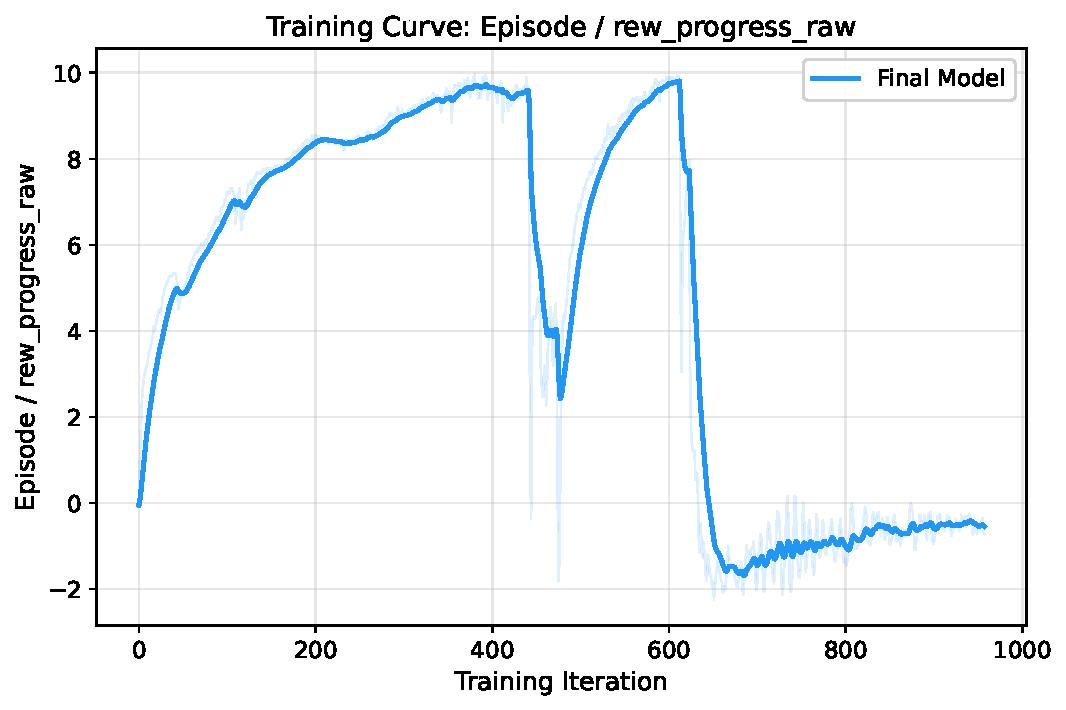
\includegraphics[width=0.48\textwidth]{figures/training/Episode_rew_progress_raw.pdf}
    \hfill
    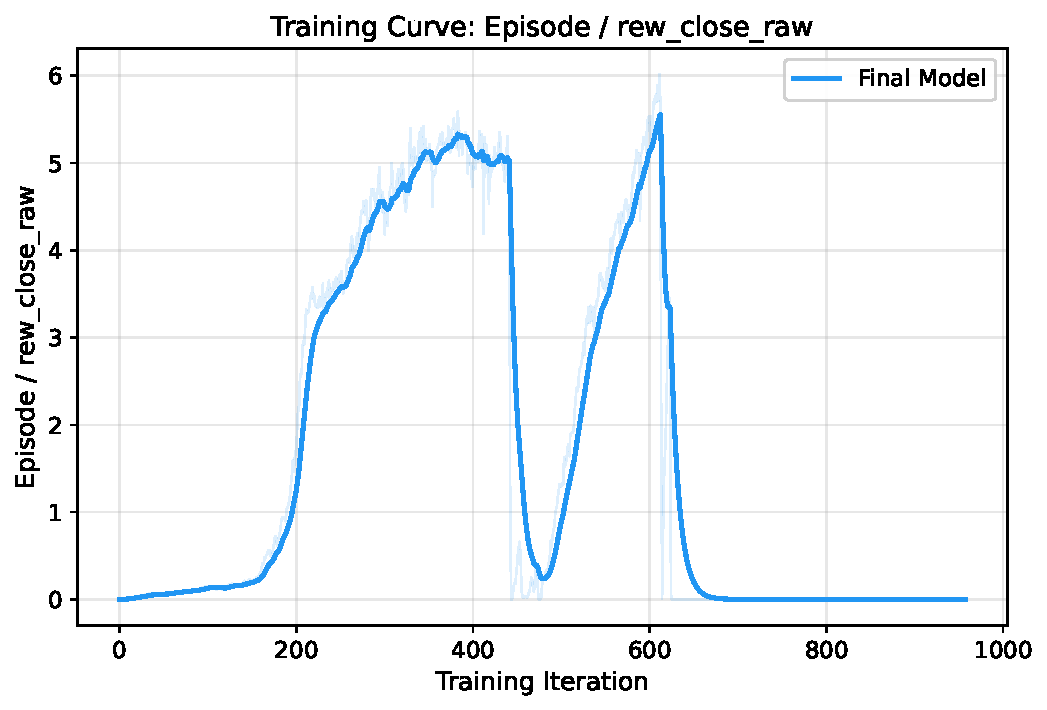
\includegraphics[width=0.48\textwidth]{figures/training/Episode_rew_close_raw.pdf}
    \caption[Fortschrittsbelohnung und Näherungsbelohnung]{Fortschrittsbelohnung
    (links) und Näherungsbelohnung (rechts). Beide Komponenten steigen mit
    zunehmender Annäherung an das Ziel.}
    \label{fig:rew_progress_close}
\end{figure}

\begin{figure}[H]
    \centering
    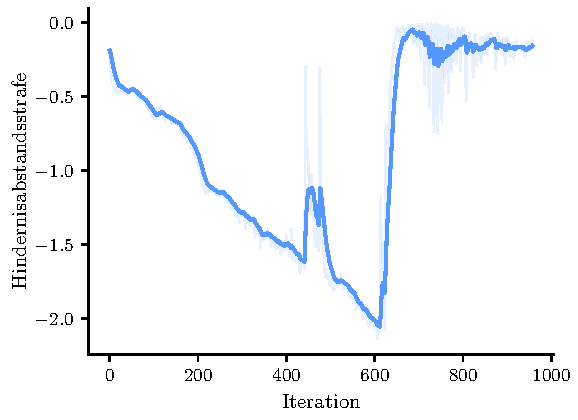
\includegraphics[width=0.48\textwidth]{figures/training/Episode_rew_obstacle_proximity_raw.pdf}
    \hfill
    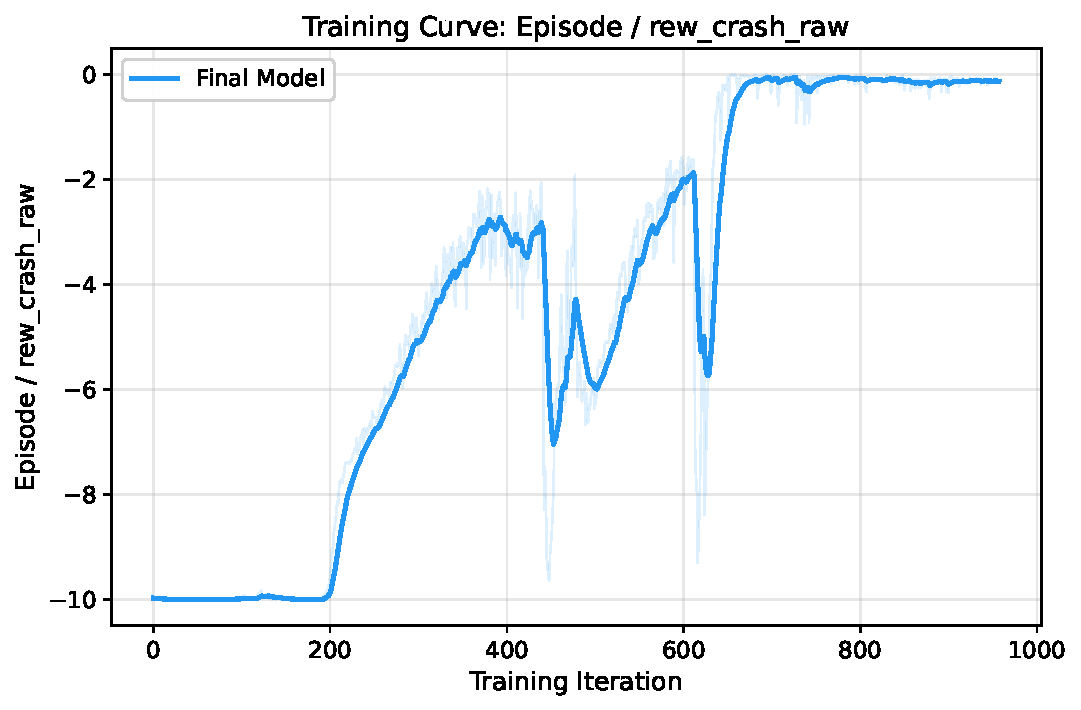
\includegraphics[width=0.48\textwidth]{figures/training/Episode_rew_crash_raw.pdf}
    \caption[Hindernisabstandsstrafe und Absturzstrafe]{Hindernisabstandsstrafe
    (links) und Absturzstrafe (rechts). Beide Strafkomponenten fallen mit
    zunehmender Kollisionsvermeidung.}
    \label{fig:rew_prox_crash}
\end{figure}

\begin{figure}[H]
    \centering
    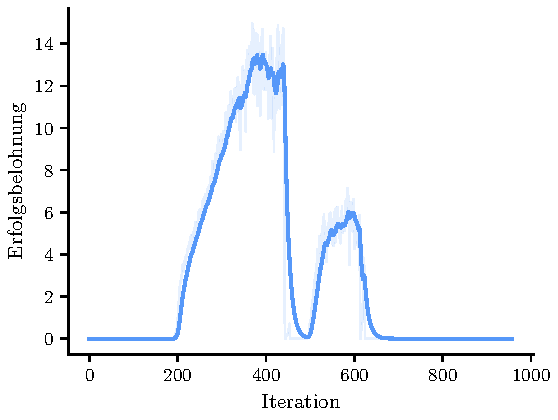
\includegraphics[width=0.48\textwidth]{figures/training/Episode_rew_success_raw.pdf}
    \hfill
    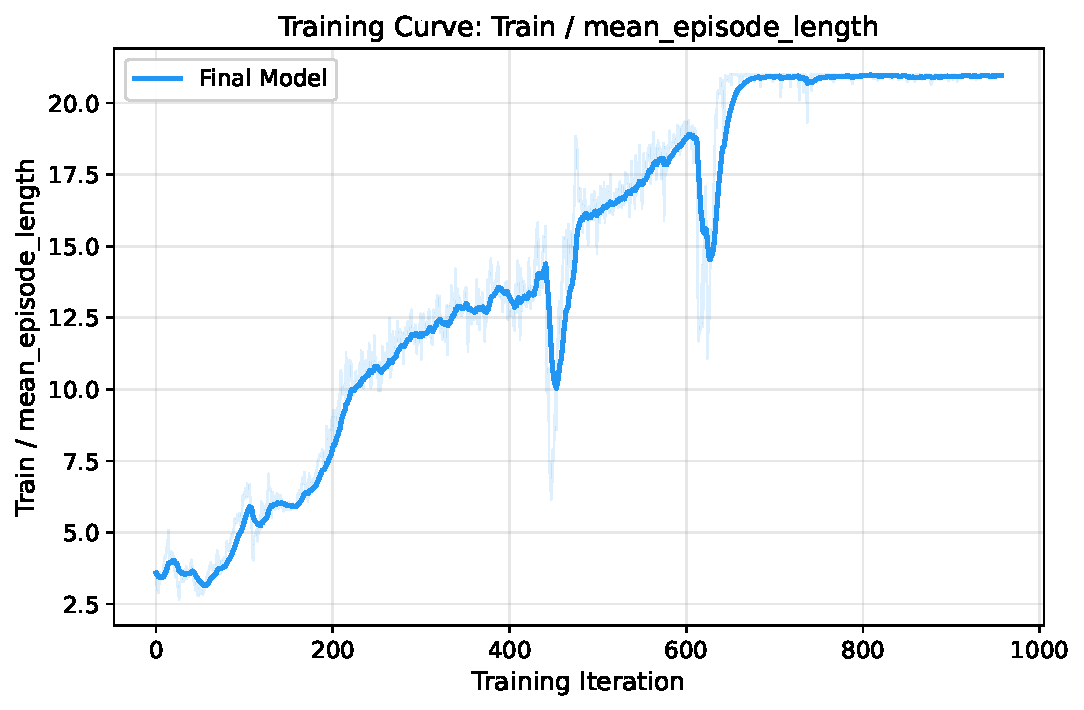
\includegraphics[width=0.48\textwidth]{figures/training/Train_mean_episode_length.pdf}
    \caption[Erfolgsbelohnung und Episodenlänge]{Erfolgsbelohnung (links) und
    mittlere Episodenlänge (rechts). Der Anstieg der Erfolgsbelohnung markiert
    den Beginn erfolgreicher Landungen. Die Episodenlänge gibt die Anzahl der
    Entscheidungsschritte pro Episode an.}
    \label{fig:rew_success_eplen}
\end{figure}

\begin{figure}[H]
    \centering
    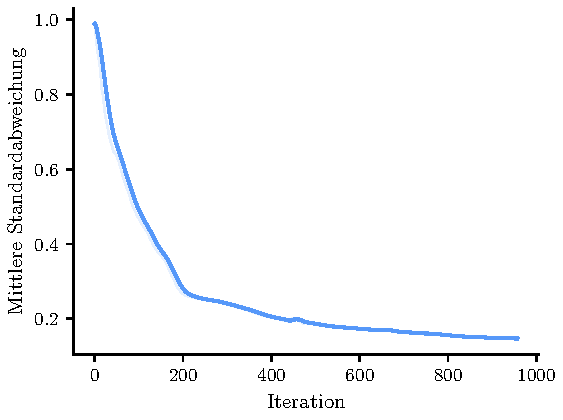
\includegraphics[width=0.48\textwidth]{figures/training/Policy_mean_std.pdf}
    \hfill
    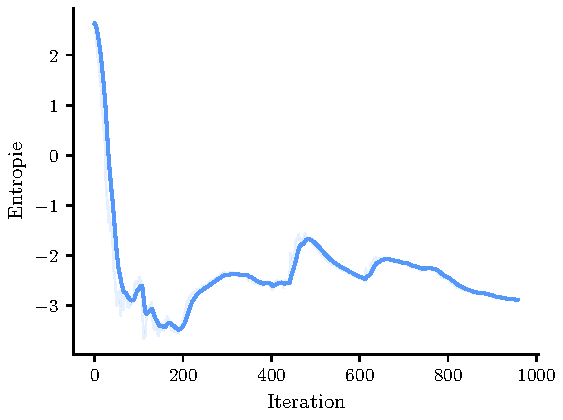
\includegraphics[width=0.48\textwidth]{figures/training/Loss_entropy.pdf}
    \caption[Standardabweichung und Entropie]{Mittlere Standardabweichung der
    Aktionsverteilung (links) und Entropie (rechts). Beide Maße fallen
    monoton und spiegeln die abnehmende Exploration wider.}
    \label{fig:rew_prox_std}
\end{figure}

\begin{figure}[H]
    \centering
    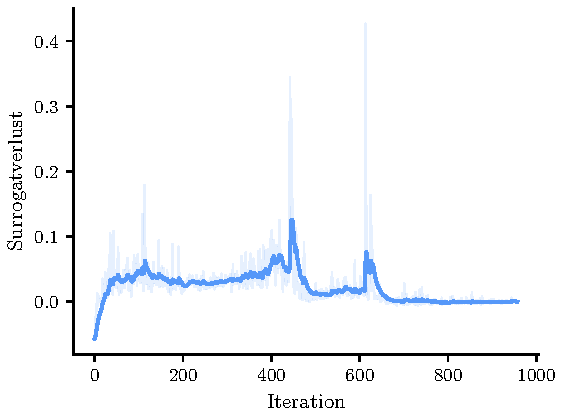
\includegraphics[width=0.48\textwidth]{figures/training/Loss_surrogate.pdf}
    \hfill
    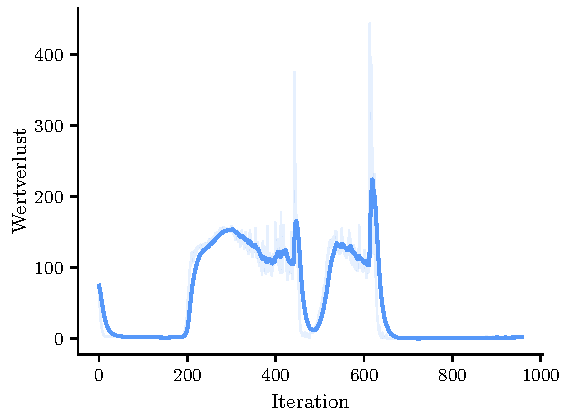
\includegraphics[width=0.48\textwidth]{figures/training/Loss_value.pdf}
    \caption[Surrogatverlust und Wertverlust]{PPO-Surrogatverlust (links) und
    Wertverlust (rechts).}
    \label{fig:loss_surrogate_value}
\end{figure}


\appsection{Standardabweichung über alle Seeds}
\label{app:std_seeds}

\begin{figure}[H]
    \centering
    
\includegraphics[width=\textwidth]{Bilder/seed_analysis/policy_std_seeds.pdf}
    \caption[Standardabweichung der Aktionsverteilung]{Mittlere
    Standardabweichung der Aktionsverteilung über alle sechs Seeds. Der
    Verlauf ist nahezu identisch und fällt von 0,99 auf circa 0,15,
    unabhängig vom jeweiligen Belohnungsverlauf. Geglättet mit EMA
    $\alpha = 0{,}9$.}
    \label{fig:policy_std_seeds}
\end{figure}


\appsection{Phase-1-Evaluationsmetriken}
\label{app:phase1_metrics}

\begin{table}[H]
  \centering
  \caption[Phase-1-Ergebnisse des RL-Agenten]{Phase-1-Ergebnisse des
  RL-Agenten ($1\,000$~Episoden, Checkpoint~400, ungesehene Hindernisse).
  Konfidenzintervalle: 95\,\%-Bootstrap (Perzentilmethode, $B = 10\,000$).
  Landezeit und Pfadeffizienz beziehen sich ausschließlich auf
  erfolgreiche Episoden ($n = 710$).}
  \label{tab:phase1_results}
  \small
  \renewcommand{\arraystretch}{1.1}
  \begin{tabular}{l r r}
    \toprule
    \textbf{Metrik} & \textbf{Wert} & \textbf{95\,\%-KI / IQR} \\
    \midrule
    Erfolgsrate                       & 71,0\,\%          & [68,2;\; 73,8] \\
    \addlinespace
    Hinderniskollision                & 28,8\,\% (288)    & [26,0;\; 31,6] \\
    Verlassen des Korridors           & 0,2\,\% (2)       & [0,0;\; 0,5] \\
    Bodenkollision                    & 0,0\,\% (0)       & — \\
    Timeout                           & 0,0\,\% (0)       & — \\
    \addlinespace
    Landezeit (Median)                & 30,0\,s            & IQR [27,0;\; 36,0] \\
    Pfadeffizienz (Median)            & 1,19               & IQR [1,13;\; 1,25] \\
    Min.\ Hindernisabstand (Mittel)   & 0,52\,m            & [0,50;\; 0,54] \\
    \bottomrule
  \end{tabular}
\end{table}


\appsection{Phase-1-Evaluationsmetriken (oberflächenbasierte Kollisionserkennung)}
\label{app:phase1_mesh_metrics}

\begin{table}[H]
  \centering
  \caption[Phase-1-Ergebnisse mit oberflächenbasierter Kollisionserkennung]{Phase-1-Ergebnisse des
  RL-Agenten mit oberflächenbasierter Kollisionserkennung ($1\,000$~Episoden,
  Checkpoint~400, ungesehene Hindernisse).
  Konfidenzintervalle: 95\,\%-Bootstrap (Perzentilmethode, $B = 10\,000$).
  Landezeit und Pfadeffizienz beziehen sich ausschließlich auf
  erfolgreiche Episoden ($n = 984$).}
  \label{tab:phase1_mesh_results}
  \small
  \renewcommand{\arraystretch}{1.1}
  \begin{tabular}{l r r}
    \toprule
    \textbf{Metrik} & \textbf{Wert} & \textbf{95\,\%-KI / IQR} \\
    \midrule
    Erfolgsrate                       & 98,4\,\%          & [97,6;\; 99,1] \\
    \addlinespace
    Hinderniskollision                & 1,2\,\% (12)      & [0,6;\; 1,9] \\
    Verlassen des Korridors           & 0,2\,\% (2)       & [0,0;\; 0,5] \\
    Bodenkollision                    & 0,0\,\% (0)       & — \\
    Timeout                           & 0,2\,\% (2)       & [0,0;\; 0,5] \\
    \addlinespace
    Landezeit (Median)                & 33,0\,s            & IQR [30,0;\; 36,0] \\
    Pfadeffizienz (Median)            & 1,19               & IQR [1,13;\; 1,25] \\
    Min.\ Hindernisabstand (Mittel)   & 0,51\,m            & [0,49;\; 0,53] \\
    \bottomrule
  \end{tabular}
\end{table}


\appsection{Phase-1-Evaluationsmetriken (RRT-Connect)}
\label{app:phase1_rrt_metrics}

\begin{table}[H]
  \centering
  \caption[Phase-1-Ergebnisse des RRT-Connect-Planers]{Phase-1-Ergebnisse des
  RRT-Connect-Planers ($1\,000$~Episoden, Checkpoint~400, ungesehene Hindernisse).
  Konfidenzintervalle: 95\,\%-Bootstrap (Perzentilmethode, $B = 10\,000$).
  Landezeit und Pfadeffizienz beziehen sich ausschließlich auf
  erfolgreiche Episoden ($n = 820$).}
  \label{tab:phase1_rrt_results}
  \small
  \renewcommand{\arraystretch}{1.1}
  \begin{tabular}{l r r}
    \toprule
    \textbf{Metrik} & \textbf{Wert} & \textbf{95\,\%-KI / IQR} \\
    \midrule
    Erfolgsrate                       & 82,0\,\%          & [79,6;\; 84,4] \\
    \addlinespace
    Hinderniskollision                & 18,0\,\% (180)    & [15,6;\; 20,4] \\
    Verlassen des Korridors           & 0,0\,\% (0)       & — \\
    Bodenkollision                    & 0,0\,\% (0)       & — \\
    Timeout                           & 0,0\,\% (0)       & — \\
    \addlinespace
    Landezeit (Median)                & 42,0\,s            & IQR [42,0;\; 48,0] \\
    Pfadeffizienz (Median)            & 1,09               & IQR [1,07;\; 1,20] \\
    Min.\ Hindernisabstand (Mittel)   & 0,48\,m            & [0,47;\; 0,49] \\
    \bottomrule
  \end{tabular}
\end{table}


\appsection{Phase-2-Evaluationsmetriken}
\label{app:phase2_metrics}

\begin{table}[H]
  \centering
  \caption[Phase-2-Ergebnisse des RL-Agenten]{Phase-2-Ergebnisse des
  RL-Agenten ($1\,000$~Episoden, Checkpoint~400, Weinberg-Transfer,
  Erfolgsradius $0{,}5$\,m).
  Konfidenzintervalle: 95\,\%-Bootstrap (Perzentilmethode, $B = 10\,000$).
  Landezeit und Pfadeffizienz beziehen sich ausschließlich auf
  erfolgreiche Episoden ($n = 104$).}
  \label{tab:phase2_results}
  \small
  \renewcommand{\arraystretch}{1.1}
  \begin{tabular}{l r r}
    \toprule
    \textbf{Metrik} & \textbf{Wert} & \textbf{95\,\%-KI / IQR} \\
    \midrule
    Erfolgsrate                       & 10,4\,\%          & [8,5;\; 12,4] \\
    \addlinespace
    Terrain-Kollision                 & 15,9\,\% (159)    & [13,6;\; 18,2] \\
    Timeout                           & 73,7\,\% (737)    & [71,0;\; 76,4] \\
    Bodenkollision                    & \multicolumn{2}{c}{entfällt (kein fester Bodenkollisions-Check)} \\
    Verlassen des Korridors           & \multicolumn{2}{c}{entfällt (kein Korridorbegrenzungsrahmen)} \\
    \addlinespace
    Landezeit (Median)                & 36,0\,s            & IQR [33,0;\; 36,0] \\
    Pfadeffizienz (Median)            & 1,07               & IQR [1,05;\; 1,09] \\
    Finale Zieldistanz (Median)       & 1,19\,m            & — \\
    Min.\ Terrain-Abstand (Mittel)    & 1,02\,m            & [0,98;\; 1,06] \\
    \bottomrule
  \end{tabular}
\end{table}


\appsection{Phase-2-Evaluationsmetriken (RRT-Connect)}
\label{app:phase2_rrt_metrics}

\begin{table}[H]
  \centering
  \caption[Phase-2-Ergebnisse des RRT-Connect-Planers]{Phase-2-Ergebnisse des
  RRT-Connect-Planers ($1\,000$~Episoden, Checkpoint~400, Weinberg-Transfer,
  Erfolgsradius $0{,}5$\,m).
  Konfidenzintervalle: 95\,\%-Bootstrap (Perzentilmethode, $B = 10\,000$).
  Landezeit und Pfadeffizienz beziehen sich ausschließlich auf
  erfolgreiche Episoden ($n = 857$).}
  \label{tab:phase2_rrt_results}
  \small
  \renewcommand{\arraystretch}{1.1}
  \begin{tabular}{l r r}
    \toprule
    \textbf{Metrik} & \textbf{Wert} & \textbf{95\,\%-KI / IQR} \\
    \midrule
    Erfolgsrate                       & 85,7\,\%          & [83,5;\; 87,9] \\
    \addlinespace
    Terrain-Kollision                 & 7,1\,\% (71)      & [5,6;\; 8,7] \\
    Timeout                           & 7,9\,\% (79)      & [6,3;\; 9,6] \\
    Bodenkollision                    & \multicolumn{2}{c}{entfällt (kein fester Bodenkollisions-Check)} \\
    Verlassen des Korridors           & \multicolumn{2}{c}{entfällt (kein Korridorbegrenzungsrahmen)} \\
    \addlinespace
    Landezeit (Median)                & 42,0\,s            & IQR [39,0;\; 48,0] \\
    Pfadeffizienz (Median)            & 0,99               & IQR [0,97;\; 1,00] \\
    Min.\ Terrain-Abstand (Mittel)    & 0,46\,m            & [0,45;\; 0,47] \\
    \bottomrule
  \end{tabular}
\end{table}


\appsection{PID-Reglerparameter}
\label{app:pid}

\begin{table}[H]
  \centering
  \caption{PID-Verstärkungen des kaskadierenden Reglers.}
  \label{tab:app_pid_gains}
  \begin{tabular}{l c c c}
    \toprule
    Regelkreis & $K_p$ & $K_i$ & $K_d$ \\
    \midrule
    Position $x$/$y$         & 1{,}0   & 0     & 0{,}7  \\
    Position $z$             & 1{,}5   & 0     & 1{,}0  \\
    Geschwindigkeit $x$/$y$  & 16{,}0  & 0     & 8{,}0  \\
    Geschwindigkeit $z$      & 100{,}0 & 2{,}0 & 10{,}0 \\
    Roll / Nick              & 6{,}0   & 0     & 3{,}0  \\
    Gier                     & 0{,}5   & 0     & 0{,}8  \\
    \bottomrule
  \end{tabular}
\end{table}



% ======================================================================
% Literaturverzeichnis
% ----------------------------------------------------------------------
% Erstellt mit biblatex aus der zugehörigen Datenbank.
% ======================================================================
\printbibliography


% ======================================================================
% Selbstständigkeitserklärung
% ======================================================================
\include{Inhalt/Erklaerung}


% ======================================================================
% Optionaler Index
% ======================================================================
% \printindex

\end{document}
